\documentclass[11pt]{article}

\usepackage[margin=1in]{geometry}
\usepackage{amsmath,amssymb,amsfonts,mathtools}
\usepackage{array}
\usepackage{enumitem}
\usepackage[capitalize]{cleveref}
\usepackage[most]{tcolorbox}
\allowdisplaybreaks[4]
\usepackage{xcolor}

\newcommand{\vbeta}{\boldsymbol{\beta}}
\newcommand{\valpha}{\boldsymbol{\alpha}}
\newcommand{\vL}{\mathbf{L}}
\newcommand{\vomega}{\boldsymbol{\omega}}
\newcommand{\vK}{\mathbf{K}}
\newcommand{\vcK}{\boldsymbol{\mathcal{K}}}
\newcommand{\vM}{\mathbf{M}}
\newcommand{\vcM}{\boldsymbol{\mathcal{M}}}
\newcommand{\vcW}{\boldsymbol{\mathcal{W}}}
\newcommand{\vB}{\mathbf{B}}
\newcommand{\vC}{\mathbf{C}}
\newcommand{\vD}{\mathbf{D}}
\newcommand{\vE}{\mathbf{E}}
\newcommand{\vg}{\mathbf{g}}
\newcommand{\ve}{\mathbf{e}}
\newcommand{\vu}{\mathbf{u}}
\newcommand{\vf}{\mathbf{f}}
\newcommand{\vkappa}{\boldsymbol{\kappa}}
\newcommand{\vphi}{\boldsymbol{\phi}}
\newcommand{\cV}{\mathcal{V}}
\newcommand{\cI}{\mathcal{I}}
\newcommand{\cQ}{\mathcal{Q}}
\newcommand{\vn}{\mathbf{n}}
\newcommand{\vm}{\mathbf{m}}
\newcommand{\vcP}{\boldsymbol{\mathcal{P}}}
\newcommand{\vxi}{\boldsymbol{\xi}}
\newcommand{\vx}{\mathbf{x}}
\newcommand{\cJ}{\mathcal{J}}
\newcommand{\NC}{N_C}
\newcommand{\NGamma}{N_{\Gamma}}
\newcommand{\vp}{\mathbf{p}}
\newcommand{\vP}{\mathbf{P}}
\newcommand{\hl}[1]{\colorbox{yellow}{#1}}
\newcommand{\cP}{\mathcal{P}}
\newcommand{\cN}{\mathcal{N}}
\newcommand{\vX}{\mathbf{X}}
\newcommand{\bvu}{\bar{\mathbf{u}}}
\newcommand{\bvA}{\bar{\mathbf{A}}}
\newcommand{\bvB}{\bar{\mathbf{B}}}
\newcommand{\bvw}{\bar{\mathbf{w}}}
\newcommand{\vA}{\mathbf{A}}
\newcommand{\bvx}{\bar{\mathbf{x}}}
\newcommand{\vN}{\mathbf{N}}
\newcommand{\vR}{\mathbf{R}}
\newcommand{\vr}{\mathbf{r}}
\newcommand{\vQ}{\mathbf{Q}}
\newcommand{\bvcA}{\overline{\boldsymbol{\mathcal{A}}}}
\newcommand{\bvcB}{\overline{\boldsymbol{\mathcal{B}}}}
\newcommand{\bvcF}{\overline{\boldsymbol{\mathcal{F}}}}
\newcommand{\bu}{\bar{u}}
\newcommand{\vPi}{\boldsymbol{\Pi}}
\newcommand{\cB}{\mathcal{B}}
\newcommand{\cE}{\mathcal{E}}
\newcommand{\vcA}{\boldsymbol{\mathcal{A}}}
\newcommand{\vcB}{\boldsymbol{\mathcal{B}}}
\newcommand{\vcF}{\boldsymbol{\mathcal{F}}}
\newcommand{\vpsi}{\boldsymbol{\psi}}
\newcommand{\vS}{\mathbf{S}}
\newcommand{\vmu}{\boldsymbol{\mu}}
\newcommand{\bvtheta}{\overline{\boldsymbol{\theta}}}
\newcommand{\vtheta}{\boldsymbol{\theta}}
\newcommand{\vzero}{\mathbf{0}}
\newcommand{\vz}{\mathbf{z}}
\newcommand{\vPhi}{\boldsymbol{\Phi}}
\newcommand{\vT}{\mathbf{T}}
\newcommand{\Deltavtheta}{\Delta\boldsymbol{\theta}}
\newcommand{\vw}{\mathbf{w}}
\newcommand{\vW}{\mathbf{W}}
\newcommand{\bvD}{\bar{\mathbf{D}}}
\newcommand{\bvC}{\bar{\mathbf{C}}}
\newcommand{\bvE}{\bar{\mathbf{E}}}
\newcommand{\bvF}{\bar{\mathbf{F}}}
\newcommand{\vs}{\mathbf{s}}
\newcommand{\vF}{\mathbf{F}}
\newcommand{\vG}{\mathbf{G}}
\newcommand{\vH}{\mathbf{H}}
\newcommand{\vPsi}{\boldsymbol{\Psi}}
\newcommand{\cF}{\mathcal{F}}
\newcommand{\btheta}{\overline{\theta}}
\newcommand{\bw}{\bar{w}}
\newcommand{\Deltabvtheta}{\Delta\overline{\boldsymbol{\theta}}}
\newcommand{\vbtheta}{\overline{\boldsymbol{\theta}}}
\newcommand{\vvarphi}{\boldsymbol{\varphi}}
\newcommand{\vI}{\mathbf{I}}
\newcommand{\Kplus}{K^{+}}
\newcommand{\Kminus}{K^{-}}
\newcommand{\vk}{\mathbf{k}}
\newcommand{\vJ}{\mathbf{J}}
\newcommand{\vKappa}{\mathbf{Kappa}}

\title{Physics-Infused Reduced-Order Modeling for Analysis of Multi-Layered Hypersonic Thermal Protection Systems With Imperfect Thermal Contacts}
\author{}
\date{}

\begin{document}
\maketitle

\begin{abstract}
    This work presents a systematic design and implementation of the physics-infused reduced-order modeling (PIROM) framework for optimal inference and reduced-order modeling of hypersonic TPS with unknown thermal contact resistances (TCRs). The PIROM framework is designed to leverage the strengths of both physics-based and data-driven modeling paradigms, by infusing physics-based models with data-driven components to enhance their predictive capabilities and generalizability. Inference heat conduction problems (IHCPs) are solved using the PIROM framework to infer TCRs from internal temperature measurements, while providing accurate predictions of transient TPS temperature dynamics under varying boundary conditions and material properties. Particularly, experimental limitations are considered in the design of the PIROM framework, including noisy observables and thermocouple placement limitations. The performance of the PIROM framework is benchmarked against traditional physics-based modeling approaches (e.g, one-dimensional FEM) and data-driven surrogate models (e.g., neural ordinary differential equations) for both inferring contact conductances and transient TPS temperature dynamics. 
\end{abstract}

\section{Introduction}

Hypersonic thermal protection systems (TPS) play a critical role in safeguarding hypersonic vehicles as they are exposed to extreme aerodynamic heating during flight. Therefore, accurate modeling and prediction of TPS behavior become essential for designing effective thermal protection strategies. Nonetheless, the highly non-linear fluid-thermal-structural interactions, temperature-dependent material property variations, and uncertainties in thermal contact resistances (TCR) at the interfaces of the TPS layers, pose significant challenges for traditional modeling approaches such as finite-element methods (FEM), as well as reduced-order (ROM) and surrogate (SM) modeling techniques.

Particularly, a critical artifact in transient reduced-order modeling of hypersonic TPS is the presence of TCRs. Due to manufacturing limitations, when two solids are brought together to form an interface, the true solid-to-solid contact area between them is generally a small fraction of the apparent area over which they meet {Minges1970}. The net effect of imperfect contact is the formation of a temperature discontinuity at the interface that is in general challenging to predict, and that significantly affects the heat transfer across the interface. The TCRs at the interfaces can vary by orders of magnitude depending on the surface roughness, contact pressure, and temperature {Minges1970,Deng2026}. This variability in TCRs can lead to significant uncertainties in the temperatures predicted by ROMs, and thus compromise the reliability of the ROMs for design and analysis of hypersonic TPS {Fang2023}. Thus, there is a critical need for modeling approaches that can effectively account for the uncertainties in TCRs while still providing accurate predictions of TPS behavior under varying conditions such as boundary conditions and material properties.

Attempts to address the challenges of modeling hypersonic TPS with unknown TCRs have been made using various approaches, ranging from traditional physics-based modeling to data-driven techniques {X}.


The objectives of this work as summarized as follows:
\begin{enumerate}
    \item Demonstrate the systematic application of PIROM to hypersonic TPS with unknown contact resistances, emphasizing on the simultaneous inference of contact conductances and hidden dynamics under varying boundary conditions and material properties.
    \item Benchmark the performance of PIROM against state-of-the-art machine learning, SciML, and traditional physics-based modeling approaches (e.g., FEM) for both inferring contact conductances and transient TPS temperature dynamics.
    \item Assess the performance of the PIROM in an experimental setting,...
\end{enumerate}
\section{Modeling of Hypersonic Thermal Protection Systems}

The following discussion presents the modeling of the transient heat conduction problem in multi-layered hypersonic thermal protection systems (TPS) with imperfect contact resistances. Moreover, three different physics-based approaches of decreasing fidelity are presented for solving the governing equations: (i) a fine three-dimensional FEM termed the \emph{full-order model} (FOM), (ii) a one-dimensional FEM with linear elements termed the \emph{one-dimensional FEM} (1D-FEM), and (iii) a lumped-mass representation of the TPS termed the \emph{lumped capacitance model} (LCM). The governing equations and their three solutions strategies are presented next.

\subsection{Governing Equations}

Consider the generic domain $\Omega\subset\mathbb{R}^{d}$ show in Fig.~\ref{fig_general_domain}. A heat flux $q_b$ (i.e., Neumann boundary condition) is prescribed on boundary $e_q$, while a temperature $T_b$ (i.e., Dirichlet boundary condition) is prescribed on boundary $e_T$, and $\partial\Omega = \cup_{i=1}^{N}\partial\Omega_i$ where $e_{iq},e_{iT}\subset\partial\Omega_i$. The transient heat conduction dynamics is governed by the following energy PDE,
\begin{subequations}
 \begin{align}
    \rho c_p \partial_t T - \nabla\cdot\left(\vk(T)\nabla T\right) &= 0, \: x\in\Omega\\
    -\vk(T)\nabla T\cdot\vn &= q_b(x,t), \: x\in e_q\\
    T(x,t) &= T_b(x,t), \: x\in e_T\\
    T(x,0) &= T_0(x), \: x\in\Omega
 \end{align}
\end{subequations}
where the density $\rho$ is constant, while the heat capacity $c_p$ and thermal conductivity $\vk\in\mathbb{R}^{d\times d}$ are temperature-dependent. The TPS domain is divided into $N_C$ non-overlapping components $\left\{\Omega_i\right\}_{i=1}^{N_C}$, where $N_{\Gamma}$ different imperfect contacts are present at the interfaces between components. For example, Fig.~\ref{fig_general_domain} contains $N_C=3$ components and $N_{\Gamma}=3$ imperfect contacts between components. Imperfect contacts translate into \emph{thermal contact resistances} (TCRs), which lead to temperature discontinuities at the interfaces between TPS layers. Therefore, large uncertainties in TCRs may have a significant impact on the overall heat transfer dynamics of TPS. The following discussion presents the simulation of hypersonic TPS under the presence of TCRs, where three different approaches of decreasing fidelity are presented: a full-order three-dimensional finite-element model (FOM), a one-dimensional FEM approximation, and a modified lumped capacitance model (LCM).

\begin{figure}
    \centering
    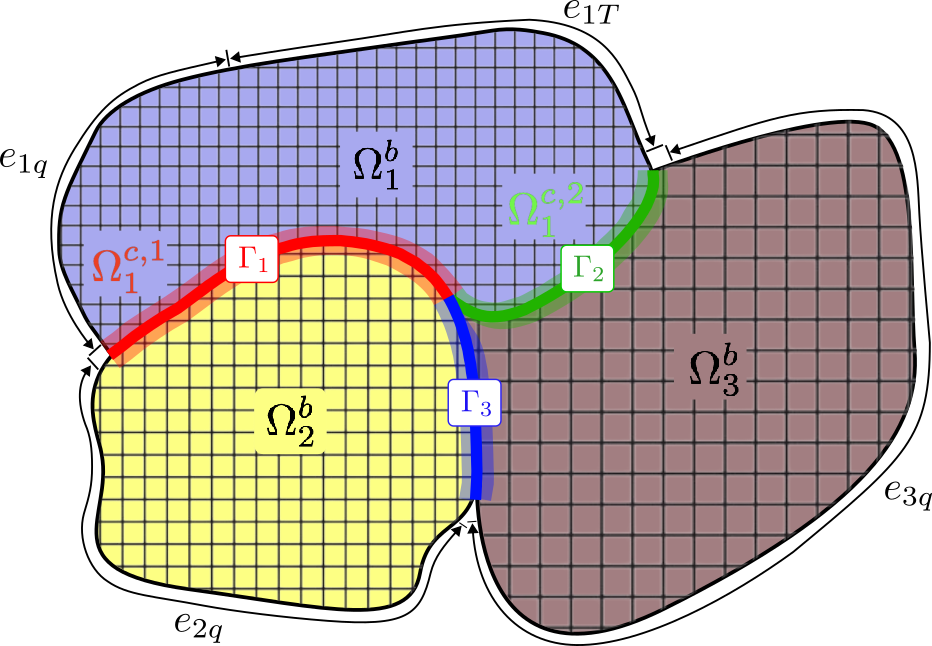
\includegraphics[width=0.99\textwidth]{./figs/modeling/domain.png}
    \caption{Schematic of the general TPS domain $\Omega$ composed of $N_C=3$ components and $N_{\Gamma}=3$ imperfect contacts between components.}
    \label{fig_general_domain}
\end{figure}

\subsection{Full-Order Model}

The FOM is obtained by spatially discretizing the governing PDE using a Discontinuous Galerkin (DG) FEM to result in a high-dimensional system of ordinary differential equations (ODEs) that captures the transient temperature dynamics of the TPS with high fidelity. As in previous work [VargasVenegas2026], the DG-FEM is chosen to describe the FOM as it: (i) provices a systematic framework for modeling multi-layered TPS with complex geometries and material properties, (ii) provides a natural framework for incorporating TCRs at the interfaces, and (iii) is amenable to systematic model reduction via coarse-graining. In Sec. [X] the FOM numerical solutions are performed using standard FEM instead, and the equivalence between DG and standard FEM is noted upon their convergence.

Consider a DG-FEM spatial discretization of the governing PDE, where the entire domain $\Omega$ is partitioned into $M$ non-overlapping elements $\left\{E_i\right\}_{i=1}^M$, where each element belong to one and only one component of the TPS. Moreover, the perfect, imperfect, Neumann, and Dirichlet boundary interfaces are denoted as $e_{ij}$, $\Gamma_{ij}$, $e_{iq}$, and $e_{iT}$, respectively. Lastly, $\left|\partial E_i\right|$ denotes the length $(d=2)$ or area $(d=3)$ of a boundary $\partial E_i$. Now, for the $i$-th element, use a set of $P$ basis functions, such as polynomials, to represent the temperature field as,
\begin{equation}
    T_i(x,t) = \sum_{p=1}^P \vphi_p(x) u_{i,p}(t),\qquad x\in E_i
\end{equation}
Without loss of generality, let the basis functions on element $E_i$ satisfy the following orthogonality condition,
\begin{equation}
    \int_{E_i}\phi_p^i\phi_q^i d\Omega = \left|E_i\right|\delta_{pq},\quad p\neq q\label{eqn_basis_functions_condition}
\end{equation}
where $\delta_{pq}$ is the Kronecker delta. Furthermore, to aid in subsequent model-order reduction derivations, choose $\phi_1^i=1$; therefore, by orthogonality, $\int_{E_i}\phi_p^i d\Omega = 0$ for $p>1$. The first basis function therefore captures the volume-averaged temperature of the element, while the remaining basis functions capture the spatially-varying temperature distributions within the element.

By standard variational procedure, e.g., [Pernet2018], the full governing equation is denoted as,
\begin{equation}
    \vA(\vu)\dot{\vu} = \vB\left(\vu\right)\vu + \vf^{(b)}(t) + \vf^{(c)}(\vu,t)
\end{equation}
where $\vu=\left[\vu_1^\top,\vu_2^\top,\dots,\vu_M^\top\right]^\top\in\mathbb{R}^{MP}$ corresponds to the DG-FEM states, $\vA$ and $\vB$ are the mass and stiffness matrices, respectively, which are functions of the temperature-dependent material properties, and $\vf^{(b)}$ and $\vf^{(c)}$ correspond to the contributions of the boundary conditions and the TCRs, respectively.

\subsection{One-Dimensional Finite-Element Model}

This approach follows a \emph{one-dimensional} FEM (1D-FEM) approach, where the governing PDE is spatially discretized using a standard FEM with linear basis functions along the thickness direction of the TPS, while the in-plane temperature gradients are neglected. This simplification is commonly used in the literature for modeling heat conduction in multi-layered TPS, since under hypersonic thermal loading, the temperature gradient along the thickness direction of the structure is significantly higher than the in-plane temperature gradients, and thus the through-thickness temperature distribution dominates the overall thermal response of the system [Gao2026].

As with the FOM, the TCR introduces additional considerations in the formulation of the 1D-FEM. 

\section{Lumped Capacitance Model with Imperfect Contacts}

This work leverages the \emph{lumped capacitance model} (LCM), a first-principle physics-based model of the TPS that captures the transient component-wise average temperature of the TPS [Incropera2011]. Nonetheless, the presence of TCRs at the interfaces introduces additional modeling considerations since the temperature drop across an interface includes, in addition to the bulk drop across the interface, a contribution from the contact resistance. The following discussion presents the formulation of the LCM for modeling the transient thermal response of the TPS with unknown TCRs, and the separation of dynamics into \emph{bulk} and \emph{contact} contributions.

\paragraph*{Bulk Dynamics} Leveraging our previous work in Ref. [VargasVenegas2026], a modified version of the LCM is leveraged in this work as the physics-based component in the PIROM. The LCM may be derived at the component level from a point of view of energy conservation, and is written as,
\begin{equation}
    \int_{\Omega_i}\rho c_{p,i}(\bar{u})\dot{\bar{u}}_i d\Omega = \sum_{j\in\cN^e_i}\int_{e_{ij}}q^{(e)}_{ij}d\Gamma + \sum_{j\in\cN_i^{c}}\int_{\Gamma_{ij}}q^{(c)}_{ij}d\Gamma + \int_{e_{iq}}q_{b}d\Gamma + \int_{e_{iT}}q_{T}d\Gamma
\end{equation}
where $q^{(e)}_{ij}$ and $q^{(c)}_{ij}$ correspond to the heat flux due to neighboring elements with perfect ($e_{ij}$) and imperfect $(\Gamma_{ij})$ interfacing surfaces, while $q_{ib}$ and $q_{iT}$ are the heat flux contributions from the Neumann and Dirichlet boundary conditions on the $e_{iq}$ and $e_{iT}$ interfaces.



The set $\cN_i$ corresponds to the neighboring components of component $i$, which are defined as those components that share an interface with component $i$. For a perfect contact between components, the heat flux $q_{ij}$ is written as $q_{ij} = G_{ij}(\bar{\vu})(\bar{u}_i - \bar{u}_j)$ where $G_{ij}(\bar{\vu})$ is the effective conductance. However, the presence of TCRs introduces an additional temperature drop across the interface, as discussed next.

\paragraph*{Contact Dynamics} Consider Fig. [X], where the interface $\Gamma_k=\partial\Omega_{l(k)}\cap\partial\Omega_{r(l)}$ is magnified to depict the governing heat transfer mechanisms. For interface $\Gamma_k$ define the average temperature on the 



The variables $\theta_i^-$ and $\theta_i^+$ represent the averaged interfacial temperatures, immediately to the left and to the right of the interface, respectively, while $z_i^-$ and $z_i^+$ represent the thermocouple measurements at distances $\delta_i^-$ and $\delta_i^+$ to the left and right of the interface, respectively. Additionally, $R_i^-$, $R_i^+$, and $R_{x,i}$ correspond to the bulk thermal resistance of the left and right layers, and the contact resistance at the interface, respectively. The total temperature drop across the interface is therefore the sum of the bulk temperature drop and the contact temperature drop, i.e.,
\begin{equation}
    \underbrace{\bar{u}_{i} - \bar{u}_{i+1}}_{\text{total lumped drop}} = \underbrace{\bigl(\bar{u}_i - \theta_i^-\bigr) + \bigl( \theta_i^+  - \bar{u}_{i+1}\bigr)}_{\text{bulk drop}} + \underbrace{\bigl(\theta_i^- - \theta_i^+\bigr)}_{\text{contact drop}}
\end{equation}
hence, the bulk drop becomes,
\begin{equation}
    \left(\bar{u}_i - \theta_i^-\right) + \left( \theta_i^+  - \bar{u}_{i+1}\right) = \left(\bar{u}_i - \bar{u}_{i+1}\right) - \Delta\theta_i 
\end{equation}
Therefore, at an interface $i\in\mathcal{I}$ with a contact resistance, the heat flux between neighboring components may be written as,
\begin{equation}
    q_{ij} = G_{ij}(\bar{\vu})\Bigl(\bigl(\bar{u}_i - \bar{u}_j\bigr) - \Delta\theta_{i}\Bigr)
\end{equation}

\begin{figure}
    \centering
    
\includegraphics[width=0.9\textwidth]{./interface.png}
    \caption{Schematic of the interface between two layers of the TPS, where the temperature drop across the interface is decomposed into a bulk drop and a contact drop.}
    \label{fig_interface}
\end{figure}






Consider the lumped-mass average temperature state,
\begin{equation}
    \vu = \left[u_1, u_2, u_3, u_4\right]^T\in\mathbb{R}^{N}
\end{equation}
and temperature-dependent lumped-capacitance matrix,
\begin{equation}
    A(\vu) = \begin{bmatrix}
        a_1(u_1) & 0 & 0 & 0 \\
        0 & a_2(u_2) & 0 & 0 \\
        0 & 0 & a_3(u_3) & 0 \\
        0 & 0 & 0 & a_4(u_4)
    \end{bmatrix}
\end{equation}
Let the external Neumann forcing be applied to the first lumped mass,
\begin{equation}
    \vf(t) = \begin{bmatrix} f(t) \\ 0 \\ 0 \\ 0 \end{bmatrix}
\end{equation}
For interfaces $i=1,2,3$, define the known \emph{bulk resistances}
\begin{equation}
    S_i(\vu)=R_i^{-}(\vu)+R_i^{+}(\vu)
\end{equation}
and the unknown contact resistance,
\begin{equation}
    R_{xi}>0,\qquad g_{xi}:=\frac{1}{R_{xi}}.
\end{equation}

The classical lumped-capacitance model with effective series resistances is,
\begin{equation}
    A\left(\vu\right)\dot{\vu} = B\left(\vu\right)\vu + \vf(t)\label{eqn_lcm}
\end{equation}
where,
\begin{equation}
    B\left(\vu\right) = \sum_{i=1}^{N-1}\frac{1}{S_i(\vu)+R_{xi}}\vK_i
\end{equation}
with standard nearest-neighbor diffusion stencils,
\begin{equation}
    \vK_1 = \begin{bmatrix}
        1 & -1 & 0 & 0 \\
        -1 & 1 & 0 & 0 \\
        0 & 0 & 0 & 0 \\
        0 & 0 & 0 & 0
    \end{bmatrix},\: \vK_2 = \begin{bmatrix}
        0 & 0 & 0 & 0 \\
        0 & 1 & -1 & 0 \\
        0 & -1 & 1 & 0 \\
        0 & 0 & 0 & 0
    \end{bmatrix},\: \vK_3 = \begin{bmatrix}
        0 & 0 & 0 & 0 \\
        0 & 0 & 0 & 0 \\
        0 & 0 & 1 & -1 \\
        0 & 0 & -1 & 1
    \end{bmatrix}
\end{equation}

The effective heat flux through interface $i$ is therefore,
\begin{equation}
    q_i = \frac{u_{i+1}-u_i}{S_i(\vu)+R_{xi}}
\end{equation}
where the temperature-drop convention is always taken as,
\begin{equation}
    \Delta u_i = u_{i+1}-u_i
\end{equation}

\subsection{Total drop = bulk drop + contact drop}

To separate bulk and contact contributions, introduce interface temperatures
\begin{equation}
    \theta_i^{+},\qquad \theta_i^{-},\qquad i=1,2,3,
\end{equation}
where $\theta_i^{-}$ and $\theta_i^{+}$ are the temperatures immediately to the left and right of contact $i$, respectively. Define the contact temperature jumps as,
\begin{equation}
    \Delta\theta_i:=\theta_i^{+}-\theta_i^{-}, \qquad i=1,2,3
\end{equation}



The total lumped-to-lumped temperature drop across interface $i$,
\begin{equation}
    u_{i+1}-u_i
\end{equation}
This total lumped-to-lumped temperature drop is the sum of the bulk drop across the interface and the contact jump across the interface,
\begin{equation}
    \underbrace{u_{i+1}-u_i}_{\text{total drop}} = \underbrace{\bigl(\theta_i^{-}-u_i\bigr)+\bigl(u_{i+1}-\theta_i^{+}\bigr)}_{\text{bulk drop}} + \underbrace{\bigl(\theta_i^{+}-\theta_i^{-}\bigr)}_{\text{contact drop}}.
\end{equation}
Hence,
\begin{equation}
    \underbrace{\left(\theta_i^- - u_i\right) + \left(u_{i+1}-\theta_i^+\right)}_{\text{bulk drop}} = \underbrace{(u_{i+1}-u_i)}_{\text{total drop}} - \underbrace{\Delta\theta_i}_{\text{contact drop}}
\end{equation}

\begin{equation}
\text{bulk drop across interface }i
=
(u_{i+1}-u_i)-\Delta\theta_i.
\label{eq:bulk_drop}
\end{equation}

Thus the lifted state is
\[
x=
\begin{bmatrix}
u\\ \Deltavtheta
\end{bmatrix}
=
\begin{bmatrix}
u_1\\u_2\\u_3\\u_4\\\Delta\theta_1\\\Delta\theta_2\\\Delta\theta_3
\end{bmatrix}
\in \mathbb{R}^{7},
\qquad
\Deltavtheta=
\begin{bmatrix}
\Delta\theta_1\\\Delta\theta_2\\\Delta\theta_3
\end{bmatrix}.
\]

\subsection{Heat-flux Continuity and DAE Formulation}

Using the adopted convention, define the bulk and contact heat fluxes as
\begin{equation}
q_i^{(b)}
=
\frac{(u_{i+1}-u_i)-\Delta\theta_i}{S_i(u)},
\qquad
q_i^{(c)}
=
\frac{\Delta\theta_i}{R_{xi}}
=
g_{xi}\Delta\theta_i.
\label{eq:q_bulk_contact}
\end{equation}

Heat-flux continuity across each interface requires
\begin{equation}
q_i^{(b)}=q_i^{(c)},
\qquad i=1,2,3,
\label{eq:flux_continuity}
\end{equation}
which yields the algebraic constraints
\begin{equation}
\frac{(u_{i+1}-u_i)-\Delta\theta_i}{S_i(u)}
-
g_{xi}\Delta\theta_i
=
0,
\qquad i=1,2,3.
\label{eq:algebraic_constraints}
\end{equation}

\subsection*{Lumped-temperature dynamics}

The four lumped energy balances yield,
\begin{subequations}
    \begin{align}
        a_1(u_1)\dot u_1 &= f(t) - q_{12}^{(b)}\\
        a_2(u_2)\dot u_2 &= q_{12}^{(b)} - q_{23}^{(b)}\\
        a_3(u_3)\dot u_3 &= q_{23}^{(b)} - q_{34}^{(b)}\\
        a_4(u_4)\dot u_4 &= q_{34}^{(b)}
    \end{align}
\end{subequations}
Substituting using the bulk heat fluxes yields,
\begin{subequations}
    \begin{align}
        a_1(u_1)\dot u_1 &= f(t) - \frac{(u_2-u_1)-\Delta\theta_1}{S_1(u)}\\
        a_2(u_2)\dot u_2 &= \frac{(u_2-u_1)-\Delta\theta_1}{S_1(u)} - \frac{(u_3-u_2)-\Delta\theta_2}{S_2(u)}\\
        a_3(u_3)\dot u_3 &= \frac{(u_3-u_2)-\Delta\theta_2}{S_2(u)} - \frac{(u_4-u_3)-\Delta\theta_3}{S_3(u)}\\
        a_4(u_4)\dot u_4 &= \frac{(u_4-u_3)-\Delta\theta_3}{S_3(u)}
    \end{align}
\end{subequations}

\subsection*{Matrix form of DAE}

Define the difference matrix,
\begin{equation}
    \vD = \begin{bmatrix}
    -1 & 1 & 0 & 0 \\
    0 & -1 & 1 & 0 \\
    0 & 0 & -1 & 1
    \end{bmatrix}, \:
    \vD u = \begin{bmatrix}
    u_2-u_1 \\
    u_3-u_2 \\
    u_4-u_3
    \end{bmatrix}
\end{equation}
Define the bulk temperature stencils,
\begin{equation}
    \vK_1 = \begin{bmatrix}
        1 & -1 & 0 & 0 \\
        -1 & 1 & 0 & 0 \\
        0 & 0 & 0 & 0 \\
        0 & 0 & 0 & 0
    \end{bmatrix},\: \vK_2 = \begin{bmatrix}
        0 & 0 & 0 & 0 \\
        0 & 1 & -1 & 0 \\
        0 & -1 & 1 & 0 \\
        0 & 0 & 0 & 0
    \end{bmatrix},\: \vK_3 = \begin{bmatrix}
        0 & 0 & 0 & 0 \\
        0 & 0 & 0 & 0 \\
        0 & 0 & 1 & -1 \\
        0 & 0 & -1 & 1
    \end{bmatrix}
\end{equation}
and the bulk jump-coupling stencils,
\begin{equation}
    \vL_1 = \begin{bmatrix}
        1 & 0 & 0 \\
        -1 & 0 & 0 \\
        0 & 0 & 0 \\
        0 & 0 & 0
    \end{bmatrix},\: \vL_2 = \begin{bmatrix}
        0 & 0 & 0 \\
        0 & 1 & 0 \\
        0 & -1 & 0 \\
        0 & 0 & 0
    \end{bmatrix},\: \vL_3 = \begin{bmatrix}
        0 & 0 & 0 \\ 
        0 & 0 & 0 \\
        0 & 0 & 1 \\
        0 & 0 & -1
    \end{bmatrix}
\end{equation}
Then,
\begin{equation}
    A(u)\dot{u} = \sum_{i=1}^{N-1}\frac{1}{S_i(u)}\Bigl(\vK_i u+\vL_i\Deltavtheta\Bigr) + \vf(t)
\end{equation}
and the algebraic constraints for heat flux continuity are written as,
\begin{equation}
    \operatorname{diag}\!\left(\frac{1}{S_1(u)},\frac{1}{S_2(u)},\frac{1}{S_3(u)}\right)\vD u - \left[\operatorname{diag}\!\left(\frac{1}{S_1(u)},\frac{1}{S_2(u)},\frac{1}{S_3(u)}\right) + G_x\right]\Deltavtheta = 0\label{eqn_algebraic_heat_flux_constraints}
\end{equation}
where
\begin{equation}
    G_x = \begin{bmatrix}
    g_{x1} & 0 & 0 \\
    0 & g_{x2} & 0 \\
    0 & 0 & g_{x3}
    \end{bmatrix}
\end{equation}
Equation \eqref{eqn_algebraic_heat_flux_constraints}, along with the lumped-temperature dynamics, defines a DAE system for the lifted state $x=[u,\Deltavtheta]$.

\subsection{DAE index reduction}

The DAE is index-reduced by differentiating the heat-flux continuity constraints with respect to time, which, for each interface $i$, yields,
\begin{equation}
    \frac{d}{dt}\left[\frac{(u_{i+1}-u_i)-\Delta\theta_i}{S_i(u)} - g_{xi}\Delta\theta_i\right] = 0
\end{equation}
The contact conductances $g_{xi}$ are assumed constant, therefore,
\begin{equation}
    \bigl(1+g_{xi}S_i(u)\bigr)\Delta\dot{\theta}_i = \bigl(\dot{u}_{i+1} - \dot{u}_i\bigr) - \frac{(u_{i+1}-u_i)-\Delta\theta_i}{S_i(u)}\dot{S}_i(u)
\end{equation}
Using the original algebraic constraint
\begin{equation}
    \frac{(u_{i+1}-u_i)-\Delta\theta_i}{S_i(u)}=g_{xi}\Delta\theta_i,    
\end{equation}
the index-reduced dynamics become,
\begin{equation}
    \boxed{
    \Delta\dot{\theta}_i = \frac{ \dot{u}_{i+1}-\dot{u}_i - g_{xi}\Delta\theta_i\,\dot{S}_i(u)}{1+g_{xi}S_i(u)}, \qquad i=1,2,3}
\end{equation}

Define
\begin{equation}
    M(u;R_x) = \begin{bmatrix}
        1+g_{x1}S_1(u) & 0 & 0 \\
        0 & 1+g_{x2}S_2(u) & 0 \\
        0 & 0 & 1+g_{x3}S_3(u)
    \end{bmatrix}
\end{equation}
and,
\begin{equation}
    \dot{S}(u) = \begin{bmatrix}
        \dot{S}_1(u) \\
        \dot{S}_2(u) \\
        \dot{S}_3(u)
    \end{bmatrix},\qquad \Deltavtheta\odot \dot{S}(u) = \begin{bmatrix}
    \Delta\theta_1\dot{S}_1(u) \\
    \Delta\theta_2\dot{S}_2(u) \\
    \Delta\theta_3\dot{S}_3(u)
    \end{bmatrix}
\end{equation}
Then, the index-reduced dynamics for the contact jumps can be written in matrix form as,
\begin{equation}
    M(u;R_x)\Delta\dot{\theta} = D\,\dot u - G_x\bigl(\Deltavtheta\odot \dot S(u)\bigr)
\end{equation}
Thus, the index-reduced lifted system is given by the coupled ODEs,
\begin{subequations}
    \begin{align}
        A(u)\dot{u} &= \sum_{i=1}^{N-1}\frac{1}{S_i(u)}\Bigl(\vK_i u + \vL_i\Deltavtheta\Bigr) + \vf(t)\\
        M(u;R_x)\Delta\dot{\theta} &= \vD\dot{u} - G_x\bigl(\Deltavtheta\odot \dot S(u)\bigr)
    \end{align}
\end{subequations}

\section{Physics-Infused Reduced-Order Modeling}

The formulation of PIROM for TPS starts by mathematically connecting the FOM, i.e., the DG-FEM, to the RPM, i.e., the LCM. This results presented in this section leverage the previous work in Ref. {X}, where a coarse-graining procedure is developed to systematically derive the LCM from the DG-FEM. Such coarse-graining procedure pinpoints the missing dynamics in the LCM when compared to DG-FEM, enabling the systematic design of a memory closure to account for residual dynamics associated with discarded spatial resolution. 

\subsection{Deriving the Reduced-Physics Model via Coarse-Graining}

As demonstrated in previous work [VargasVenegas2026], the LCM can be viewed as a special case of the DG-FEM, where the mesh partition is extremely coarse, and the trail and test functions are piece-wise constants. In this setting, the LCM becomes a coarse zeroth-order DG-FEM with the inverse of thermal resistance chosen as the element-wise penalty factors. In this work, the presence of unknown TCRs motivates the design of a coarse-graining procedure that explicitly accounts for the presence of interfaces with unknown contact conductances, which are not captured by the LCM. 

\subsubsection{Coarse-Graining of States}

Consider a DG-FEM as in Eq. [X] for $M$ elements, and a LCM as in Eq. [X] for $N$ components with $N_{\Gamma}$ imperfect interfaces; clearly, $M\gg N$. Define the sets of indices $\cV_j$, $\cF_i^-$, and $\cF_i^+$, corresponding to the elements contained in component $j$, and the elements adjacent to interface $i$ on the negative and positive sides, respectively. Formally, the sets are defined as,
\begin{subequations}
    \begin{align}
        \cV_j &= \{i: E_i\subset\Omega_j\}\\
        \cF_i^- &= \{j\in\{1,2,\dots,M\}\:|\: \Gamma_i\cap\partial E_j\neq\emptyset, E_j\subset\Omega_i^{-}\}\\
        \cF_i^+ &= \{j\in\{1,2,\dots,M\}\:|\: \Gamma_i\cap\partial E_j\neq\emptyset, E_j\subset\Omega_i^+\}
    \end{align}
\end{subequations}
where $\Gamma_r=\partial\Omega_i^{-}\cap\partial\Omega_i^{+}$ is the imperfect interface between the minus $\Omega^{-}_i$ and plus $\Omega_i^{+}$ components. To aid in the subsequent derivations, introduce a new variable $\vw=\left[\vw_1^\top,\vw_2^\top,\dots,\vw_K^\top\right]=\left[\vw^{-},\vw^{+}\right]^\top\in\mathbb{R}^{KP}$, where $\vw_i$ corresponds to the DG-FEM states of element $i$, and $\vw^{-}\in\mathbb{R}^{K^{-}P}$ and $\vw^{+}\in\mathbb{R}^{K^{+}P}$ correspond to the DG-FEM states of the elements adjacent to the imperfect contact interfaces on the negative and positive sides, respectively. Note that $K = K^- + K^+$, where $K^-$ and $K^+$ are the number of elements adjacent to the imperfect contact interfaces on the negative and positive sides, respectively. Clearly, $M>K$, since the total number of elements is much larger than the number of elements adjacent to the imperfect contact interfaces.


Therefore, the volume and left-and-right interface averages for component $j$ and interface $r$ are given by,
\begin{subequations}
    \begin{align}
        \bar{u}_j &= \frac{1}{\left|\Omega_j\right|}\sum_{i\in\cV_j}\int_{E_i} \vphi^\top\vu_i d\Omega_i = \frac{1}{\left|\Omega_j\right|}\sum_{i\in\cV_j}\left|E_i\right|\vvarphi_i^{j\top}\vu_i, \: j=1,\ldots,N\\
        \btheta_r^{-}(t) &= \frac{1}{\left|\Gamma_r\right|}\sum_{m\in\cF_r^-}\int_{\Gamma_{rm}} \vphi_m^\top\vw_m d\Gamma_r=\sum_{m\in\cF_r^{-}}\alpha_{mr}^{-}\vmu_{mr}^{\top}\vw_{mr}^{-}, \: r=1,\ldots,N_{\Gamma}\\
        \btheta_r^{+}(t) &= \frac{1}{\left|\Gamma_r\right|}\sum_{m\in\cF_r^+}\int_{\Gamma_{rm}} \vphi_m^\top\vw_m d\Gamma_r=\sum_{m\in\cF_r^{+}}\alpha_{mr}^{+}\vmu_{mr}^{\top}\vw_{mr}^{+}, \: r=1,\ldots,N_{\Gamma}
    \end{align}
\end{subequations}
where the orthogonal basis functions are defined as $\vvarphi_i^j=\left[1,0,\dots,0\right]\in\mathbb{R}^{P}$. Moreover, $\alpha_{mr}^{-} = \frac{\left|\Gamma_{mr}\right|}{\left|\Gamma_r\right|}$ and $\alpha_{mr}^{+} = \frac{\left|\Gamma_{mr}\right|}{\left|\Gamma_r\right|}$ correspond to the fractions of the interface segment $\Gamma_{mr}$ with respect to the total interface $\Gamma_r$, $\vw_{mr}^{-}$ and $\vw_{mr}^{+}$ correspond to the DG-FEM states of the element $E_m$, which is adjacent to the imperfect interface $\Gamma_{r}$ with $r=1,2,\dots,N_{\Gamma}$ on the negative and positive sides, respectively, and $\vmu_{mr} = \frac{1}{\left|\Gamma_{mr}\right|}\int_{\Gamma_{mr}} \vphi^{\top}_m d\Gamma_{mr}\in\mathbb{R}^{P}$. Moreover, the $\Gamma_{rm} = \Gamma_r\cap\partial E_m$, and $\left|\Gamma_{rm}\right|$ is the point $(d=2)$ or area $(d=3)$ of the interface segment $\Gamma_{rm}$.

Conversely, given the average temperatures of the $N_C$ components, as well as the average minus-and-plus temperatures on the two sides of the $N_{\Gamma}$ different imperfect interfaces, the DG-FEM states may be written as,
\begin{subequations}
    \begin{align}
        \vu_i &= \sum_{k=1}^{N_C}\vvarphi_i^k\bar{u}_k + \delta\vu_i,\quad i=1,2,\dots,M\\
        \vw_{ir}^{-} &= \sum_{k=1}^{N_{\Gamma}}\vpsi_k^{r-}\btheta_k^{-} + \delta\vw_{ir}^{-},\quad i\in\cF_r^{-},r=1,2,\dots,N_{\Gamma}\\
        \vw_{ir}^{+} &= \sum_{k=1}^{N_{\Gamma}}\vpsi_k^{r+}\btheta_k^{+} + \delta\vw_{ir}^{+},\quad i\in\cF_r^{+},r=1,2,\dots,N_{\Gamma}
    \end{align}\label{eqn_element_states}
\end{subequations}
where $\vpsi_k^{r\pm}=\vzero\in\mathbb{R}^{P}$ if $k\neq r$, so that the average minus-and-plus temperatures on the two sides of the imperfect contact interface $\Gamma_r$ only contribute to the states of the elements adjacent to such interface, and $\delta\vu_i$, $\delta\vw_{ir}^{-}$, and $\delta\vw_{ir}^{+}$ correspond to the residuals between the DG-FEM states and the reconstructed states from the average temperatures.

Collectively, Eq.\cref{eqn_element_states} can be written in matrix form as,
\begin{subequations}
    \begin{align}
        \vu &= \vPhi\bar{\vu} + \delta\vu,\quad \bvu=\vPhi^{\dagger}\vu\\
        \vw &= \vPi\bar{\vtheta} + \delta\vw,\quad \bvtheta=\vPi^{\dagger}\vw
    \end{align}
\end{subequations}
where $\vPhi\in\mathbb{R}^{MP\times N_C}$ is a matrix of $M\times N_{C}$ blocks, with the $(i,j)$-th block as $\vvarphi_i^j$, $\vPhi^{\dagger}\in\mathbb{R}^{N_{C}\times MP}$ is the left inverse of $\vPhi$, with the $(i,j)$-th block as $\vvarphi_i^{j\dagger}=\frac{|E_i|}{|\Omega_j|}\vvarphi_i^{jT}$ and $\delta\vu$ is the collection of deviations from the average temperature. Moreover,
\begin{equation}
    \vPi = \begin{bmatrix}
        \vM & \vzero\\
        \vzero & \vN
    \end{bmatrix},\quad \vPi^{\dagger} = \begin{bmatrix}
        \vM^{\dagger} & \vzero\\
        \vzero & \vN^{\dagger}
    \end{bmatrix}
\end{equation}
where $\vM\in\mathbb{R}^{K^{-}P\times\NGamma}$, $\vN\in\mathbb{R}^{K^{+}P\times\NGamma}$ correspond to the lifting matrices from the minus-and-plus interface average temperatures $\bvtheta^{-},\bvtheta^{+}\in\mathbb{R}^{\NGamma}$. By their definitions, the projection matrices satisfy,
\begin{subequations}
    \begin{align*}
        \vPhi^{+}\vPhi &= \vI, & \vPhi^{+}\delta\vu  &= \vzero\\
        \vM^{+}\vM     &= \vI, & \vM^{+}\delta\vw^{-} &= \vzero\\
        \vN^{+}\vN     &= \vI, & \vN^{+}\delta\vw^{+} &= \vzero
    \end{align*}
\end{subequations}


\subsubsection{Coarse-Graining of Dynamics}

Next, the coarse-graining operator for the LCM dynamics is selected as in previous work [VargasVenegas2026], which consists of a Galerkin projection of the DG-FEM dynamics onto the subspace spanned by the coarse-grained states described by the average temperatures. The critical result of the coarse-graining procedure is that the LCM dynamics can be written in the following form,

\subsection{Formulation of Reduced-Order Model}

The Mori-Zwanzig (MZ) formalism is an operator-projection technique use to derive ROMs for high-dimensional dynamical systems, especially in statistical mechanics and fluid dynamics [Parish2017,Stinis2017,Parish2025]. It provides an exact reformulation of the full-order dynamics in terms of a subset of resolved states. The proposed PIROM is subsequently developed based on such reformulation.



\section{Bulk-only Mori--Zwanzig Memory Closure}

The purpose of the closure is to account for the unresolved dynamics in the LCM, while leaving the contact-jump dynamics unchanged. Accordingly, the 


Accordingly, write the Projected Generalized Langevin Equation (PGLE) for the lumped-temperature dynamics,
\begin{equation}
    A(\vu)\dot{\vu} = \sum_{i=1}^{N-1}\frac{1}{S_i(\vu)}\left(\vK_i u + \vL_i\Deltavtheta\right) + \vf(t) + \int_{t_0}^{t}\vkappa(t,s,u,\vf;\Theta)ds
\end{equation}
Now, ensure the designed memory modifies only the bulk conductances, i.e.,
\begin{equation}
    \vkappa\in\text{span}\left\{\vK_1 u(t), \vK_2 u(t), \vK_3 u(t), \vL_1 \Deltavtheta_1(t), \vL_2 \Deltavtheta_2(t), \vL_3 \Deltavtheta_3(t)\right\}
\end{equation}
which leads to,
\begin{equation}
    \vkappa(t,s,u,\vf;\Theta) \approx \sum_{j=1}^{m}\kappa_j(t,s,u,\vf;\Theta)\vcP_j
\end{equation}
where,
\begin{equation}
    \vcP_j = \sum_{i=1}^{N-1}\frac{1}{S_i(u)}\vp_{ij}
\end{equation}

Now, define the memory variables as,
\begin{equation}
    \beta_j(t) = \int_{t_0}^{t}\kappa_j(t,s,u,\vf;\Theta)ds
\end{equation}
then,
\begin{equation}
    \int_{t_0}^{t}\vkappa(t,s,u,\vf;\Theta)ds = \sum_{j=1}^{m}\beta_j(t)\vcP_j
\end{equation}
It follows that,
\begin{equation}
    \sum_{j=1}^{m}\beta_j(t)\vcP_j = \sum_{j=1}^{m}\beta_j(t)\sum_{i=1}^{N-1}\frac{1}{S_i(u)}\vp_{ij} = \sum_{i=1}^{N-1}\frac{1}{S_i(u)}\left(\sum_{j=1}^{m}\vp_{ij}\beta_j(t)\right) = \sum_{i=1}^{N-1}\frac{1}{S_i(u)}\vP_i\vbeta
\end{equation}
Then, the memory correction to the LCM dynamics leads to the following modified lumped-temperature dynamics,
\begin{equation}
    A(\vu)\dot{\vu} = \sum_{i=1}^{N-1}\frac{1}{S_i(\vu)}\left(\vK_i u + \vL_i\Deltavtheta + \vP_i\vbeta\right) + \vf(t)
\end{equation}

Now, let,
\begin{equation}
    \kappa_i\left(t,s,\vu,\vf;\Theta\right) = e^{-\lambda_j(t-s)}\left(q_j^\top\phi(\vu(s)) + r_j^\top \psi(\vf(s))\right)
\end{equation}
such that the memory variables are given by,
\begin{equation}
    \vbeta(t) = \int_{t_0}^{t}e^{-\Lambda(t-s)}\left(Q^\top\phi(\vu(s)) + R^\top \psi(\vf(s))\right)ds
\end{equation}

The hidden dynamics are now given by,
\begin{equation}
    \dot{\vbeta} = -\Lambda\vbeta + Q^\top\phi(\vu) + R^\top \psi(\vf)
\end{equation}
and in state-space form, the hidden dynamics are,
\begin{equation}
    \dot{\vbeta} = -\Lambda\vbeta + Q^\top\phi(\vu) + R^\top \psi(\vf)
\end{equation}
The full lifted and closed system is given by,
\begin{subequations}
    \begin{align}
        A(\vu)\dot{\vu} &= \sum_{i=1}^{N-1}\frac{1}{S_i(\vu)}\left(\vK_i \vu + \vL_i\Deltavtheta + \vP_i\vbeta\right) + \vf(t)\\
        M(\vu;R_x)\dot{\Deltavtheta} &= \vD\dot{\vu} - G_x\bigl(\Deltavtheta\odot \dot S(\vu)\bigr)\\
        \dot{\vbeta} &= -\Lambda\vbeta + Q^\top\phi(\vu) + R^\top \psi(\vf)
    \end{align}
\end{subequations}

\begin{figure}
    \centering
    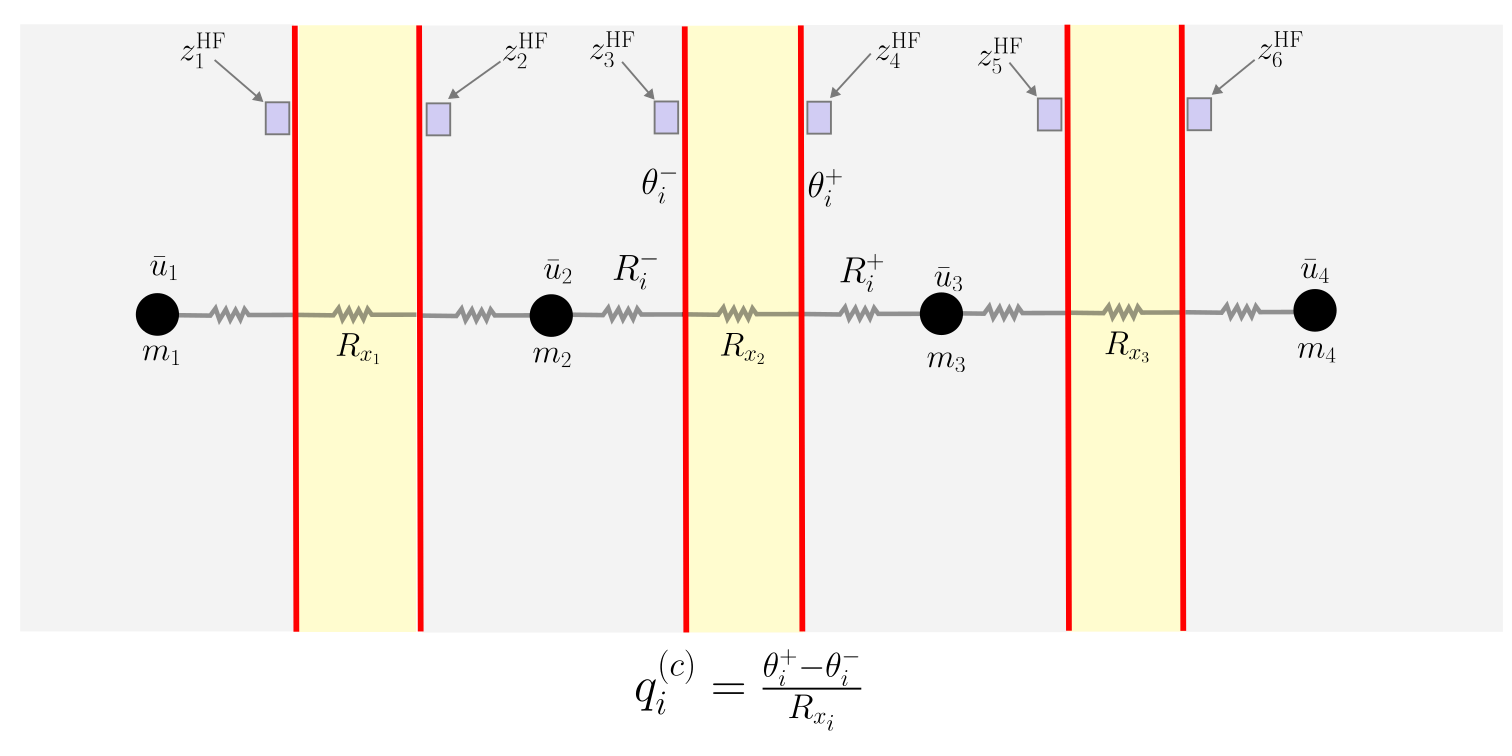
\includegraphics[width=0.9\textwidth]{./experiment.png}
\end{figure}

\section{Application to Thermal Protection Systems}

In this section, the proposed PIROM approach is applied to modeling a four-layered hypersonic TPS with unknown contact resistances, and is compared against a representative physics-based model, i.e., FEMs, and data-driven surrogate model, i.e., a neural ordinary differential equation (NODE) model. The performance of the models is assessed in terms of their ability to infer the TCRs, and to predict the transient temperature dynamics under varying boundary conditions and material properties. The configuration of the TPS, problem parametrization, optimal model design for inference, and numerical results are presented next.

\subsection{Problem Description and Parametrization}


\subsection{Model Selection}



\subsubsection{One-Dimensional Finite-Element Model}

In Section~\ref{sec:1dfem}, the 1D-FEM was introduced as utilizing linear basis functions (LBFs). These LBFs have favorable behavior when put in weak form, yielding simple stiffness and mass matrices that captures the heat transfer within material blocks and the imperfect interfaces between said blocks. However, the 1D-FEM also has the added benefit of being a first-order model; consequently, by leveraging the pair of LBFs on each side of a respective material block, the temperature at any given sensor position within the block can be easily computed via a weighted average. 

Consider the example presented in Fig.~\ref{fig:lbf_demo}, where each of the sensors are perturbed from their respective interfaces by distance $\delta$. The temperature of $z_1^{\text{HF}}$ when the temperatures on the left and right side of the first material block are $u_l$ and $u_r$ respectively is then given by
\begin{equation}
    u = u_l \cdot \frac{L-\delta}{L} + u_r \cdot \frac{\delta}{L}
\end{equation}
where $L$ is the thickness of the material block in question. By computing the weighted average of every sensor with respect to the two edge temperatures on either side, the sensor temperatures can be found regardless of the distance $\delta$ in which they are perturbed.

To examine the ability of the 1D-FEM in inferring the gap TCRs, the model will be tested in a range of experiments with two varying parameters: noise level and perturbation distance, $\delta$. For varying noise level, the high fidelity sensor readings will be injected with random Gaussian noise to corrupt the temperature signals. These sensors will then be denoised using a weak form kernel ridge regression framework \cite{kreider2026} prior to TCR training; the subsequent denoising should clean and smooth the signal, but may introduce some biases that could interfere with the inferred conductances. In response, several seeds will be evaluated for each experiment (i.e., noise level and sensor placement) --- allowing for the analysis of the overall behavior of adding noise to the system, and neglecting the erratic residue of any single seed performance. Doing so should make the evolution of TCR inference error with respect to increasing noise level clear. 

Additionally, six different sensor perturbation distances will be evaluated, or $\delta_i$ for $i=1,2,\dots,6$. These perturbations range from 0\% - 20\% of the block length $L$, with higher $i$ values corresponding to more extreme displacements of the sensors away from their respective interfaces. By sweeping a range of sensor positions from perfect to extremely perturbed placement, the trend of how conductance inference error is affected by moving the sensors away from their interfaces will be clear. 

The mean error across the ensemble is presented in Fig.~\ref{fig:cond_mean}, where the 1D-FEM model occupies the first row. It is immediately apparent that the dominant error mode of TCR inference is the sensor position, as error significantly increases as the sensor is perturbed further away from the interface. Such behavior is likely a byproduct of the LBFs, which can only accurately predict the sensor temperature readings within a small distance of the interfaces. Most of this error originates from the sensor in Acusil, whose low conductance produces an asymptotic curve that is difficult to approximate with LBFs alone. Similarly, the error increases slightly as the noise level increases, an artifact of the small biases introduced by the noise/denoise framework that shift the inferred TCR solution.

The standard deviation error for the same ensemble is illustrated in Fig.~\ref{fig:cond_std}, where the noise level is a major source of variation. Observe the negligible STD of the no-noise case where all ensembles produce essentially identical solutions, while the moderate- and high-noise cases produce steadily increasing STDs as a result of the denoising. Since more extreme noises may introduce similarly behaving biases, different seeds can produce greatly varying conductance errors. Note that at further sensor positions the perturbation error dominates the that of the noise significantly, resulting in less STD as the sensor moves further and further away (but still higher mean error). 

To summarize, the 1D-FEM performs exceptionally well when the sensor is near-perfectly placed with no significant noise. However, at large displacements or high noise levels this error rises quite significantly, an artifact of both the diminishing accuracy of the LBFs and the biases introduced by the denoising algorithm. 


\begin{figure}[htbp]
    \centering
    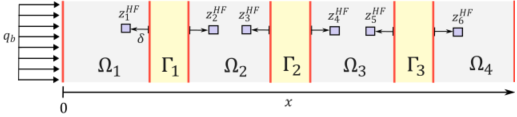
\includegraphics[width=0.8\linewidth]{figs/modeling/1D_FEM_Offset.png}
    \caption{Experimental setup with arbitrary sensor displacement, $\delta$, applied to each of the six sensors.}
    \label{fig:lbf_demo}
\end{figure}

\begin{enumerate}
    \item Discuss sensor placement and how it is done for this specific system (i.e. LBFs)
    \item Tradeoff for $C$ vs $\delta$ vs $\mathrm{SNR}$ (however, this might be best placed in the appendix with the main takeaways in the main document)
\end{enumerate}










\subsubsection{Lumped Capacitance Model}

The lumped capacitance models (LCMs) from Section~\ref{sec:lcm}, which are contrarily based in a finite-volume model, are rooted differently. Rather than leveraging LBFs to formulate a first-order model like the 1D-FEM, the LCMs operate as a zeroth-order model; that is, the only known values are the average block temperatures, and all other information must be subsequently deduced. Consequently, the approach of computing the temperature is more elaborate, consisting of recomputing effective conductances. 

Consider the demonstrative experiment presented in Fig.~\ref{fig:lcm_demo}, where a pair of sensors on either side of an interface are shown. By adjusting the $\delta$ sensor position, the effective resistance across a gap can be computed --- by moving the sensor away from the interface, the calculation must not only account for the gap resistance, but also the resistance of the block between the sensor and the interface. Consequently, the corrected resistance ensures the flux is accurate, correcting the temperatures jump in temperature across the gap and ensuring the inferred conductance is accurate. 

For perfect sensor placement, the resistance across the gap is simply $R_{x_i}$. However, as the sensor is moved away from the interface, one must account for the resistances in either material block for a proper IHCP. Thus, it is imperative to adjust the temperature jump across the gap; as heat flux is constant across the material blocks and gap interfaces, this is quite intuitive. Consider
\begin{equation}
    q = \frac{\Delta T}{R_{\text{eff}}}
\end{equation}
where the flux is given by the temperature jump across a gap with effective resistance $R_\text{eff}$. Since the flux across the interface itself will be equal to the flux through the material block and gap, the temperature difference at the new sensor positions can be computed through their relation. For $\Delta \theta$ and $\Delta z$ representing the temperature difference for the perfect and perturbed sensor placement respectively, the relation is
\begin{equation}
    \frac{\Delta z}{R_{x_1} + R_1^- + R_1^+} = \frac{\Delta \theta}{R_{x_i}} 
\end{equation}
which yields the corrected temperature jump as
\begin{equation}
    \Delta z = \Delta \theta \left[1+\frac{R_1^- + R_1^+}{R_{x_i}}\right]
\end{equation}
This framework shows how finite-volume methodology can be leveraged to compute the temperatures at the new sensor locations. As an added sanity check, if the sensor placement is perfect, $R_i^-=R_i^+=0$, which would yield $\Delta z = \Delta \theta$.

Similarly to the 1D-FEM, the LCM will be examined on its ability to infer the gap TCRs. However, in addition to testing the noise levels and perturbation distance, the refinement of the model will also be analyzed. For instance, the most coarse LCM can have four elements, one for each block --- this is denoted as LCM 4. However, the number of elements can be greater than four as well. Consider an LCM with six elements (i.e., LCM 6) which can be distributed to the four material blocks. A naive way of handling this is to place the two extra elements in random blocks, but a more structured framework is to place both extra blocks in Acusil. As Acusil has a significantly smaller conductivity --- and thus a larger temperature gradient --- the zeroth-order approximation would be the most inadequate here. Therefore, for LCM models with five or more elements, the extra elements will be isolated to the first material block where they can improve tracking of the Acusil temperature profile near the sensor. To supplement this framework, a spline can also be fit for the two elements nearest to the sensor in the Acusil layer, similar to flux reconstruction. This way the component averages can be further leveraged to improve sensor temperature approximations as $\delta$ perturbs the sensor with respect to the elements. 

By varying the noise level, sensor position, and LCM discretization, the mean errors in TCR inference can be generated as shown in Fig.~\ref{fig:cond_mean}. Observe that LCM 4 performs roughly the same as the 1D-FEM in terms of sensor placement, likely due to its similar discretization; without more elements in the Acusil layer, the temperature approximation of the sensor further from the interface is inadequate, producing a poorly inferred conductance value. However, for finer discretized models (e.g., LCM 5 and so on), the error is much smaller and more uniform, an artifact of the better sensor approximation. However, between these finely discretized models, there is not much improvement; that is, there is no real improvement from putting more than two elements in Acusil, as these two already map the temperature gradient quite well. Finally, in terms of noise level, the errors are similar to 1D-FEM for all models --- error increases slightly as the noise level increases, likely due to the biases that get introduced through the noise/denoise workflow. 

Similarly, the standard deviations for the error in inferred conductances is shown in Fig.~\ref{fig:cond_std}. Similar to 1D-FEM, the standard deviation increases as a function of noise level, with moderate noise having higher deviation than no noise, and high noise more than both. However, contrarily to the 1D-FEM and LCM 4, the finely discretized models have more uniform standard deviations. This is likely due to their overall low error, which maintains the noise level as a dominant error mode as opposed to the sensor placement in the coarser models. 

\begin{figure}[htbp]
    \centering
    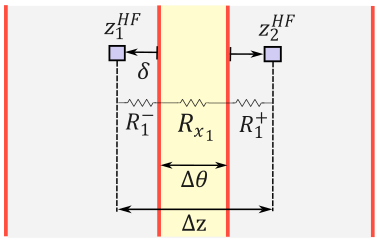
\includegraphics[width=0.4\linewidth]{figs/modeling/LCM_Demo.png}
    \caption{Demonstrative example of an arbitrary sensor displaced from its respective interface position, showing the varying effective resistance with increasing $\delta$.}
    \label{fig:lcm_demo}
\end{figure}

\begin{enumerate}
    \item Discuss sensor placement and how it is done for this specific system (i.e. moving indices in FEM)
    \item Tradeoff for $C$ vs $\delta$ vs $\mathrm{SNR}$ (however, this might be best placed in the appendix with the main takeaways in the main document)
\end{enumerate}




\subsubsection{Remarks}

With the previous analysis of the 1D-FEM and LCMs, the best choice in training for PIROM is clearly LCM 5. In Fig.~\ref{fig:cond_mean}, it is apparent that the finer models have constantly negligible error regardless of sensor position. And while there is no further improvement in error for even finer models (e.g., LCM 6-8), there is a considerable increase in runtime effort. LCM 5, which only has 5 elements, remains computationally tractable while still displaying the benefit of additional elements in Acusil. Furthermore, LCM 5 displays steady behavior across noise levels, and only sees a comparable rise in standard deviation with moderate noise compared to the other models. 

Finally, the moderate noise case is the best case to train the PIROM on, since it permits for the analysis of the effects of noise on the system while maintaining a noise intensity similar to that of real sensors. Additionally, it shows the effects of noise while still being physical; the increase in mean and deviation error rise slightly as expected, but they are still tractable for a solver. While the models were able to handle the high noise case, the intensity is quite a bit more extreme than is reasonable and is meant as more of a demonstrative example of the limitations of the model and the trend of the models with gradually increasing noise. 

\begin{figure}[htbp]
    \centering
    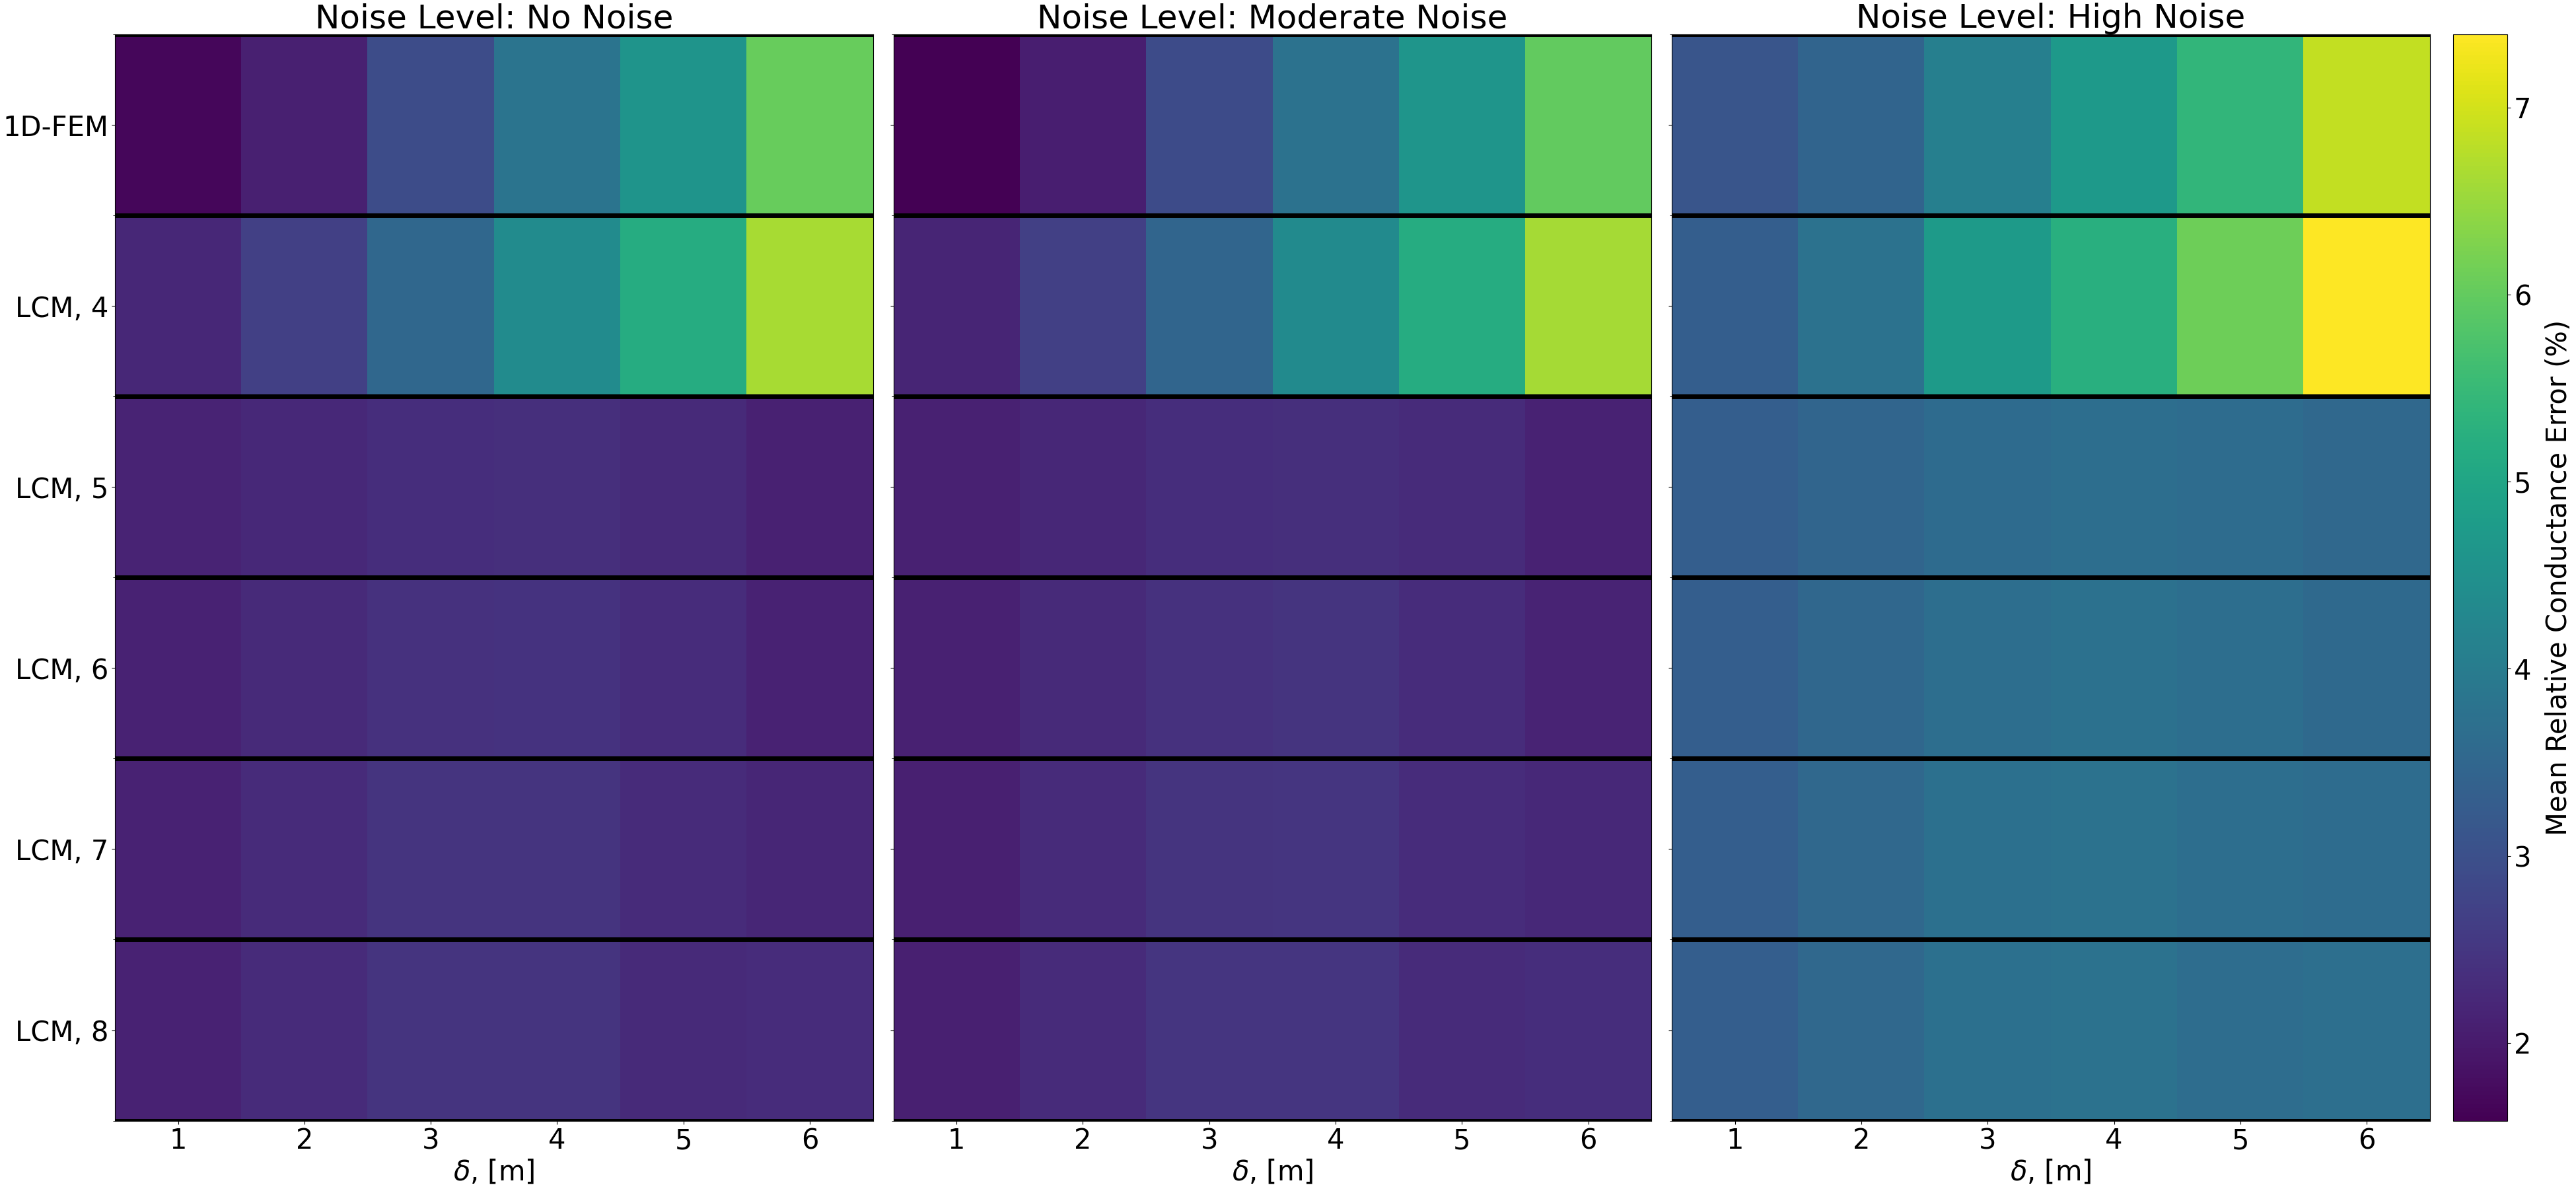
\includegraphics[width=0.99\textwidth]{./figs/results/cond_mean.png}
    \caption{Mean relative error of the inferred conductance values across a range of experiments and model selections. }
    \label{fig:cond_mean}
\end{figure}

\begin{figure}[htbp]
    \centering
    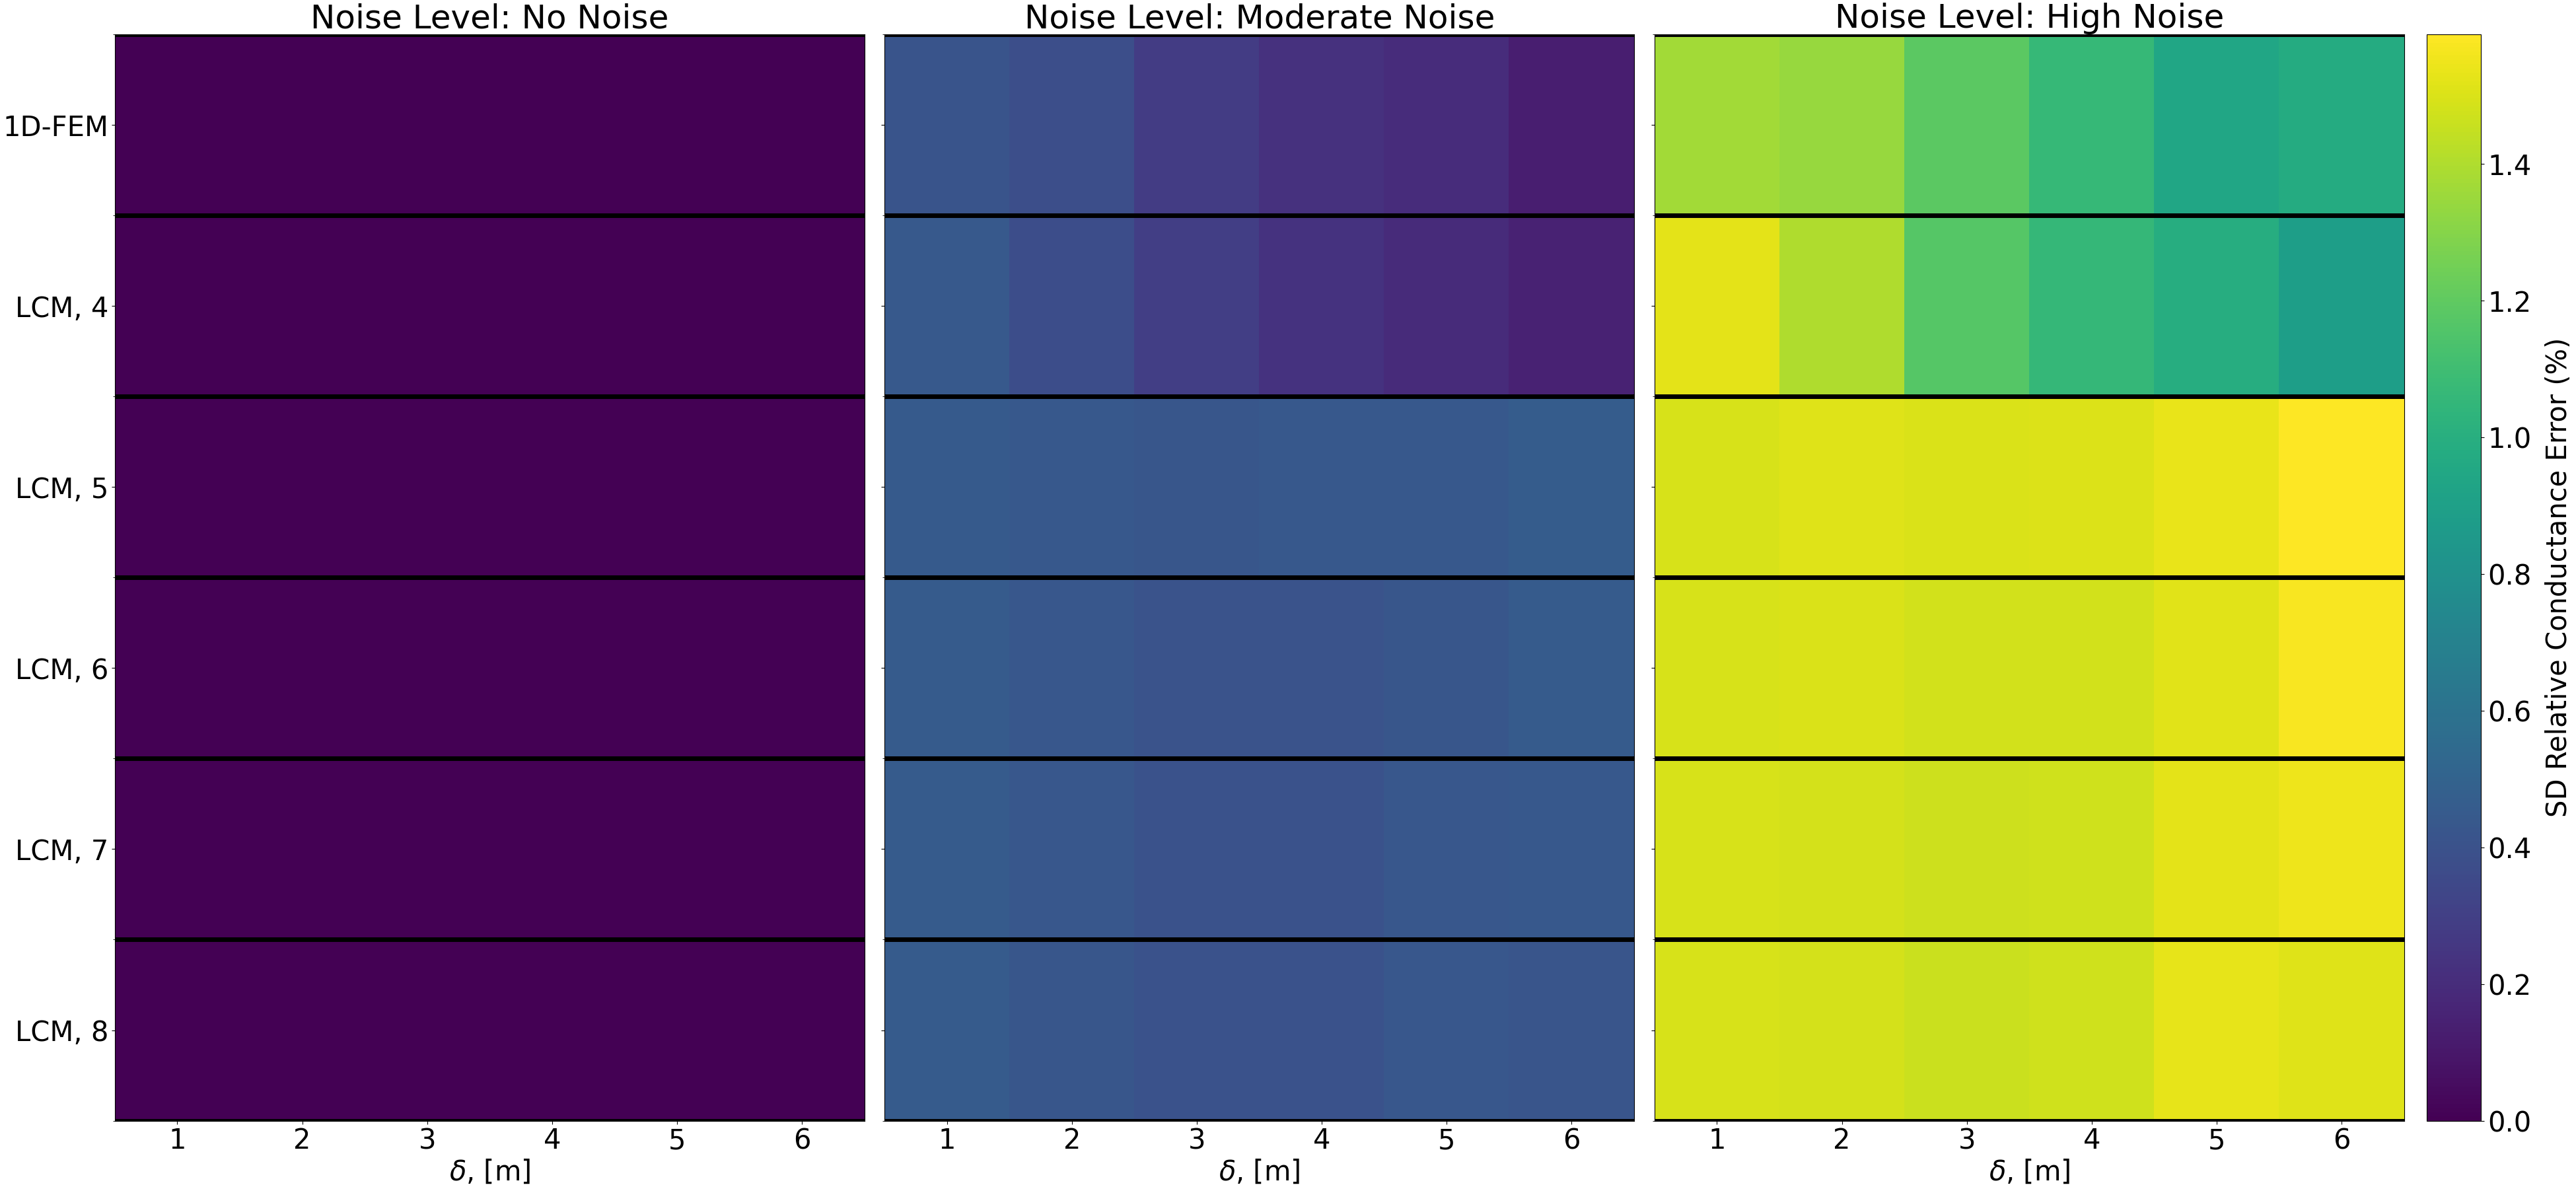
\includegraphics[width=0.99\textwidth]{./figs/results/cond_sd.png}
    \caption{The standard deviation of the relative error for the inferred conductance values from a range of experiments and model selections. }
    \label{fig:cond_std}
\end{figure}

\begin{enumerate}
    \item What model won? E.g. Model A with Noise B performed the best
    \item All else should perhaps be placed in the appendix, with this section only highlighting what model we will compare the PIROM to (to reduce total number of combinations and overall noise in the paper)
\end{enumerate}
\subsubsection{Model Performance on Transient-Dominated Timescale}

For the experiments conducted in the previous sections, the timescale was fixed and sufficiently long; in other words, the simulation time in which the models ran for was extensive enough to ensure the heat applied on the boundary condition was able to propagate through the entirety of the system. Through this, the inferred conductance inherently satisfies the steady-state effects, of whose error would dominate the cost function used to train. However, such a result brings to question the transient effects. When the timescale is short enough where the initial transients dominates --- that is, times where heat has not been able to fully penetrate the system --- the inferred conductances should have higher error as the system tries to compensate for effects it can not fully observe yet. 

Consider Fig.~\ref{fig:char_time}, which shows the error in each inferred conductance as the timescale of the simulation is altered. Observe that there is a certain simulation timescale in which the relative error drops below an adequately low threshold, which perfectly coincides with the effective characteristic time of each of the gaps. In other words, the error drops off the moment where the flux reaches the sensor located immediately after each of the respective gaps. This finding is meaningful; the time needed to infer the conductance of a gap is only the time it takes for heat to travel to the sensors on either side of the gap. Therefore, the framework does not directly necessitate steady-state, but merely must be able to observe the temperatures on either side of the gap to read the physics across it. 

For the remainder of the study, the timescale will remain adequately large to ensure sufficient heat penetration through the system; as the PIROM will mainly focus on improved tracking of sensor readings, its ability to improve transient and steady-state effects is non-trivial. However, through these results, the framework is proven capable of inferring material properties within significantly reduces timescales --- even ones which are still dominated by transients --- as long as there is observation on either side of the gap in question. 

\begin{figure}[htbp]
    \centering
    
\includegraphics[width=0.99\textwidth]{./figs/results/char_time.png}
    \caption{Evolution of error in inferred conductance as a function of simulation timescale.}
    \label{fig:char_time}
\end{figure}

\subsection{PIROM Results}
\subsubsection{PIROM Optimization}
\begin{enumerate}
    \item Hidden dynamics
    \item TCR
    \item Training costs
    \item Generalization (DONE BELOW)
    \item HS Graph??
\end{enumerate}



\subsubsection{BC Generalization}

For the nominal experiment, the boundary condition (i.e., the flux applied on the edge of the TPS) is constant throughout the simulation. However, in a real experiment, this is not always true; there are small fluctuations in the boundary conditions that the PIROM must continue to track. To do so, a sinusoidal contribution will be added to the forcing applied to the TPS. 

Consider the flux component applied to the edge of the TPS given by
\begin{equation}
    q = \sigma \cdot \left[1+\sin(\omega t)\right]
\end{equation}
where $\sigma$ and $\omega$ represent the magnitude and periodic frequency of the forcing respectively. Previously, $\omega$ is zero, signifying a constant signal. However, by randomly sampling $\omega$, a periodic element can perturb the signal while still maintaining grounding in the same general vicinity of the nominal forcing. 

The results of such perturbation are shown in Fig.~\ref{fig:track_err}, where the NRMSE of PIROM is quite significantly lower than that of both the LCM and FEM. This is an artifact of the improved tracking of the PIROM through the learned hidden states, which as expected, extend to other boundary conditions without further training. This is advantageous as only the nominal boundary conditions (i.e., constant flux) must be explicitly learned by PIROM, and the learned hidden states can be implicitly applied to any set of boundary conditions and show major improvement. A further advantage of this is warm starting; even if the error is not adequately low, it provides a much better starting point for training than cold starting would, significantly decreasing runtime for a subsequent training instance. 

\subsubsection{Material Generalization}

Another important application to test is material generalization. At high temperatures, material properties may carry more uncertainty and in practice, may not exactly match the properties that the PIROM was trained on. Thus, PIROM having the capability to extend to slightly perturbed properties is imperative in ensuring its improved tracking retains accuracy in high temperature supersonic environments. 

To model this, the material properties can be formulated as
\begin{equation}
    m^{(p)} (\bar{T}) = m^{(n)}(\bar{T}) + 0.5\Delta m^{(n)}\left[ \alpha_0 \bar{T} + \alpha_1 \sin(\alpha_2 \pi \bar{T})\right]
\end{equation}
where $m^{(p)}$ and $m^{(n)}$ are the perturbed and nominal material properties respectively, $\bar{T}$ is the normalized temperature given by $\bar{T} = \frac{T - T_\text{min}}{T_\text{max}-T_\text{min} }$, and $\xi = [\alpha_0, \alpha_1, \alpha_2]$ are the random parameters sampled to perturb the material properties.
Such a model succeeds in keeping material properties true at low temperatures, but allowing larger perturbations as temperature continues to climb. The generated perturbations are illustrated in Fig.~\ref{fig:pert_mats}, where sufficient deviation from the nominal properties is demonstrated. 

\begin{figure}[htbp]
    \centering
    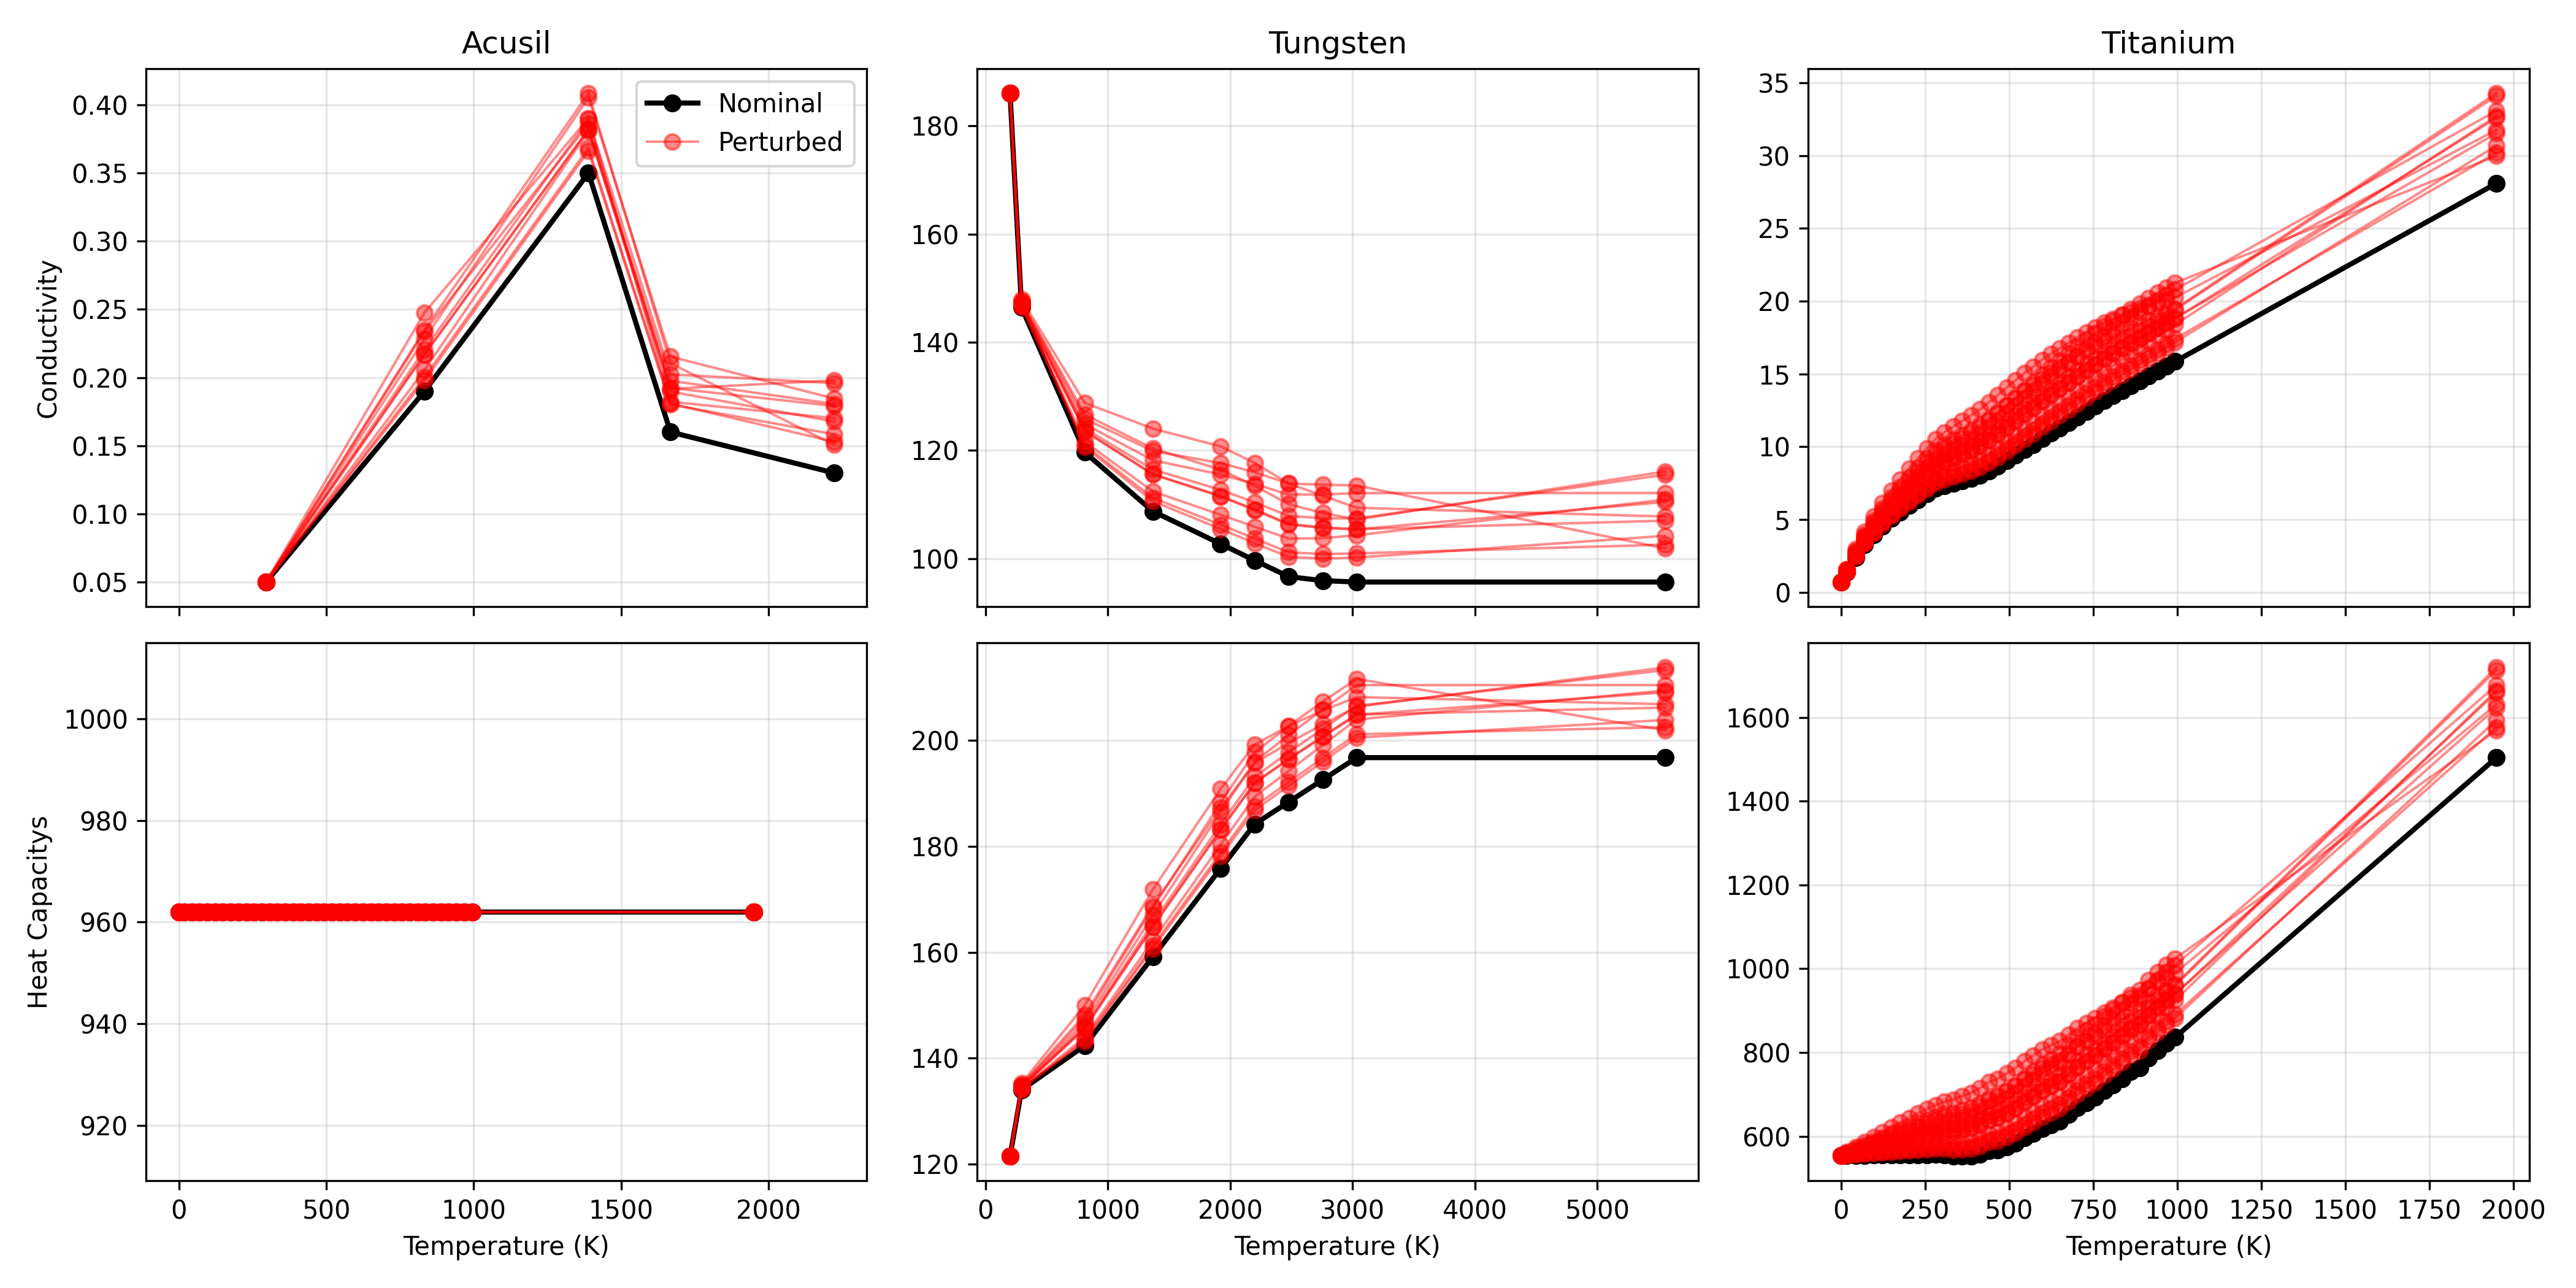
\includegraphics[width=0.9\textwidth]{./figs/modeling/pert_mats.png}
    \label{fig:pert_mats}
\end{figure}

\subsubsection{TCR Generalization}
\subsubsection{Thickness Generalization}
\subsubsection{Compounded Generalization}

\subsubsection{Extreme Thickness Generalization}

\begin{figure}[htbp]
    \centering
    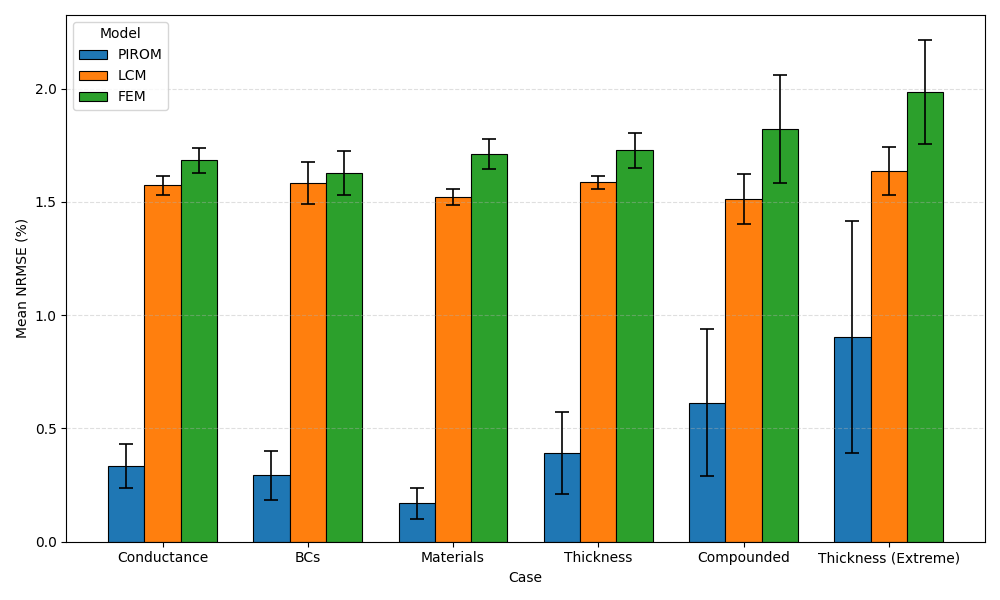
\includegraphics[width=0.9\textwidth]{./figs/results/tracking_error.png}
    \caption{Mean NRMSE of sensor tracking for each of the generalization cases. }
    \label{fig:track_err}
\end{figure}
\section{Concluding Remarks}

The main conclusion of this work are as follows,
\begin{enumerate}
    \item A one-way physics-data PIROM design is found to successully infer the unknown TCRs and hidden dynamics simulatneously. During inference, X and Y orders of magnitude in \emph{training efficiency} are obtained relative to the FOM and 1D-FEM forward models, while X and Y orders of magnitude in \emph{evaluation efficiency} 
    
    X and Y orders of magnitude in \emph{training efficiency} are obtained relati
    
    successfully infers the unknown TCRs and hidden dynamics simultaneously, offering X and Y orders of magnitude in \emph{training efficiency}, as well as X and Y
    
    relative to the FOM and 1D-FEM based model, while X and Y orders of magnitude in \emph{evlauation efficiency} 
    
    and X and Y orders of magnitude in \emph{evaluation efficiency}
    
    TCRs from noisy thermocouple 
    
    framework successfully learns a ROM for the prediction of the temperature dynamics of the TPS, while simultaneously inferring the unknown contact conductances with errors of less than X\% on noisy data with SNR of up to Y dB.
    \item The PIROM outperforms the state-of-the-art data-driven, NN-based SciML, and traditional FEM modeling approaches for inferring contact conductances, as well as for predicting the temperature dynamics for OOD configurations.
    \item Model bias is found to significantly affect the 
\end{enumerate}
\section{Appendix}

This appendix provides the technical details of the main text. 

\subsection{Lumped Capacitance Model}

The TPS is divided into $N$ components with $M$ elements. For component $i$, define $\Omega_i$ as the spatial domain of the component, and $\partial\Omega_i$ as the boundary of the component. For each interface between two components, define $l(i)$ and $r(i)$ as the left and right components that form the interface, respectively. 

For interface $i$, define $\Gamma_i=\partial\Omega_{l(i)}\cap\partial\Omega_{r(i)}$,
\begin{subequations}
    \begin{align}
        \theta_i^{-} (t) &= \frac{1}{\left|\Gamma_i\right|}\int_{\Gamma_i} T^{-}_h(x,t)d\Gamma,\\
        \theta_i^{+}(t) &= \frac{1}{\left|\Gamma_i\right|}\int_{\Gamma_i} T^{+}_h(x,t)d\Gamma\\
        \Delta\theta_i(t) &= \theta_i^{-}(t) - \theta_i^{+}(t)
    \end{align}
\end{subequations}
Define the trace operators,
\begin{subequations}
    \begin{align}
        C_i^{-}\vu &= \frac{1}{\left|\Gamma_i\right|}\int_{\Gamma_i} \sum_{j=1}^{N_u} u_j(t)\phi_j(x)d\Gamma,\\
        C_i^{+}\vu &= \frac{1}{\left|\Gamma_i\right|}\int_{\Gamma_i} \sum_{j=1}^{N_u}u_j(t)\phi_j(x)d\Gamma
    \end{align}
\end{subequations}
Stacking all the $N_{\Gamma}$ interfaces, define the trace extraction operator as,
\begin{equation}
    \vPsi^+ = \begin{bmatrix}
        C_1^{-} - C_1^{+}\\
        \vdots\\
        C_{N_{\Gamma}}^{-} - C_{N_{\Gamma}}^{+}
    \end{bmatrix}\in\mathbb{R}^{N_{\Gamma}\times MP}
\end{equation}
where $M$ is the number of elements and $P$ is the number of basis functions per element. Therefore, it follows that,
\begin{equation}
    \vs(t) = \vPsi^+\vu(t)
\end{equation}
Thus,
\begin{equation}
    \vPi^+ = \begin{bmatrix}
        \vPhi^+ \\ 
        \vPsi^+
    \end{bmatrix}
\end{equation}

Introduce the lifting matrix,
\begin{equation}
    \vPsi\in\mathbb{R}^{MP\times N_{\Gamma}}
\end{equation}
such that,
\begin{equation}
    \vPhi^+\vPsi = \vzero,\quad \vPsi^+\vPsi = \vI
\end{equation}

Note that $\Phi\bvu$ contributes $E_{\Gamma}\bvu$ to the interface jump, therefore the state decomposition can be written as,
\begin{equation}
    \vu = \vPhi\bvu + \vPsi\left(\Deltavtheta - E_{\Gamma}\bvu\right) + \delta\vu = \tilde{\vPhi}\bvu + \vPsi\Deltavtheta + \delta\vu
\end{equation}
where $\tilde{\vPhi} = \vPhi - \vPsi E_{\Gamma}$, and $\delta\vu$ is the deviation from the average temperature in the components.

\subsection{Coarse-Graining Example}

Consider the three-layered TPS shown in Fig. [X] with three components $\left\{\Omega_j\right\}_{j=1}^3$ and three contact interfaces $\left\{\Gamma_k\right\}_{k=1}^3$. The set of elements for each component, and on the minus and plus sides of each interface are defined as,
\begin{subequations}
    \begin{align}
        \cV_j &= \left\{m\in\{1,\ldots,M\}:E_m\subseteq\Omega_j\right\},\\
        \cF_k^{-} &= \left\{m\in\{1,\ldots,M\}:E_m\cap\Gamma_k\neq\emptyset, E_m\subseteq\Omega_{l(k)}\right\},\\
        \cF_k^{+} &= \left\{m\in\{1,\ldots,M\}:E_m\cap\Gamma_k\neq\emptyset, E_m\subseteq\Omega_{r(k)}\right\}
    \end{align}
\end{subequations}
where $\Omega_{l(k)}$ and $\Omega_{r(k)}$ are the left and right components that form the interface $\Gamma_k$, respectively, with $\Gamma_k = \partial\Omega_{l(k)}\cap\partial\Omega_{r(k)}$.

\end{document}